% M. S. Tsoeu (2011), University of Cape Town <mohohlo.tsoeu@uct.ac.za>

% This is a project report templace document created for EEE4022FS students at the University of Cape Town.
%
% This file should be is processed with ``pdflatex`` and might need a few modifications if a different processor is chosen.


\documentclass[a4paper,12pt]{report}

%Include packages you need to use here

\usepackage[top = 1in, bottom = 1in, left = 1in, right = 1in]{geometry}
\usepackage{graphicx}
\usepackage{fancyhdr}
\usepackage{amsmath, amsthm, amssymb}
\usepackage{lastpage}
\usepackage{subfigure}
\usepackage{lscape}
\usepackage{hyphenat}
\usepackage{setspace}
\usepackage{hyperref}

% Include page formatting here. 
\parskip = 6mm
\parindent = 0mm
\renewcommand{\headrulewidth}{0pt}
\rhead[]{\thesection}
\lhead[\thechapter]{}


\begin{document}
	
	% This section formats the title page of the Report.
	\thispagestyle{empty}
	{\Huge \begin{center}
			% Modify the line below to insert your title.
			Short Term Load Forecasting 
			\hrule 
			% Modify the line below to insert your subtitle.
			{\Large Using Machine learning and Artificial Intelligence}
	\end{center}}
	
	\vskip 5mm
	\begin{center}
		
\includegraphics[scale = 1]{images/UCT.jpg}
	\end{center}
	
	\vskip 5mm
	\begin{center}
		Presented by:\\
		Blessed Mukundi Mangena 		% Insert your name here
	\end{center}
	
	\vskip 10mm
	\begin{center}
		Prepared for:\\
		Professor Komla Folly\\ 		% Insert your supervisor's name here.
		Dept. of Electrical and Electronics Engineering\\University of Cape Town
	\end{center}
	
	
	\vskip 10mm
	\begin{center}
		Submitted to the Department of Electrical Engineering at the University of Cape Town in partial
		fulfilment of the academic requirements for a Bachelor of Science degree in Electrical and Computer Engineering
		
	\end{center}
	
	
	\vskip 5mm
	\begin{center}{\bf \today}
	\end{center}
	
	\newpage
	\thispagestyle{empty}
	\mbox{}
	\newpage
	
	\onehalfspacing
	\nohyphens{
	\thispagestyle{empty}
	\vskip 40mm
		
		
		% Please leave the declaration as it is (Standard UCT declaration).
		{\Large Declaration}\\
		\hrule
		
		\vskip 10mm
		\begin{enumerate}
			\item I know that plagiarism is wrong. Plagiarism is to use another's work and pretend that it is one's
			own.
			\item I have used the IEEE convention for citation and referencing. Each contribution to, and quotation in,
			this report from the work(s) of other people has been attributed, and has been cited and
			referenced.
			\item This report is my own work.
			\item I have not allowed, and will not allow, anyone to copy my work with the intention of passing it off
			as their own work or part thereof.
		\end{enumerate}
		\vskip 10mm
		Signature:\ldots\ldots\ldots\ldots\ldots\ldots\ldots\ldots\ldots 
		\\M. S. T\v soeu 		% Chante this line to your name.
		\vskip10mm
		Date:\ldots\ldots\ldots\ldots\ldots\ldots\ldots\ldots\ldots\ldots .
	}
		\newpage
		\thispagestyle{empty}
		{\Large Terms of Reference}\\
		\hrule
		
		The terms of reference page is an agreement between yourself and your supervisor outlining what is expected of you in your final year project. Please make sure that this is discussed and written at the beginning of your thesis project. 
		
		
		\fancyfoot[C]{\thepage}
		\pagestyle{plain}
		\newpage
		\pagenumbering{roman}
		{\Large Acknowledgments}\\
		\hrule
		Make relevant acknowledgements to people who have helped you complete or conduct this work, including sponsors or research funders.
		
		
		\newpage
		
		{\Large Abstract}\\
		\hrule
		
		% Place your abstract here.
		\begin{itemize}
			\item Open the {\bf Project Report Template.tex} file and carefully follow the comments (starting with \%).
			\item Process the file with {\bf pdflatex}, using other processors may need you to change some features such as graphics types.
			\item Note the files included in the  {\bf Project Report Template.tex} (with the .tex extension excluded). You can open these files separately and modify their contents 
			or create new ones.
			\item Contact the latex namual for more features in your document such as equations, subfigures, footnotes, subscripts \& superscripts, special characters etc.
			\item I recommend using the {\bf kile} latex IDE, as it is simple to use.
		\end{itemize}
		
		
		\newpage
		\tableofcontents
		
		%\newpage
		%\listoffigures
		
		%\newpage
		%\listoftables
		
		% Page formatting, to place section titles as headers of odd pages and Chapter titles as headers of even pages.
		\newpage
		\fancyhead[RE,LO]{}
		\fancyhead[LE]{\leftmark}
		\fancyhead[RO]{\rightmark}
		\pagestyle{fancy}
		
		\pagenumbering{arabic}
		
		% THe files included below are .tex files containing the respective chapters these are already created in this package and you can add to or modify them.
		\chapter{Introduction}

\section{Background to the study}
A very brief background to your area of research. Start off with a general introduction to the area and
then narrow it down to your focus area. Used to set the scene .
\section{Objectives of this study}
\subsection{Problems to be investigated}
Description of the main questions to be investigated in this study.
\subsection{Purpose of the study}
Give the significance of investigating these problems. It must be obvious why you are doing this study
and why it is relevant.

\section{Scope and Limitations}
Scope indicates to the reader what has and has not been included in the study. Limitations tell the
reader what factors influenced the study such as sample size, time etc. It is not a section for excuses as
to why your project may or may not have worked.

\section{Plan of development}
Here you tell the reader how your report has been organised and what is included in each
chapter.

{\bf I recommend that you write this section last. You can then tailor it to your report.}

		

\chapter{Literature Review \label{litReview}}
\subsection{Introduction}
An odd power surge phenomenon was recognized during the 2008 Olympics in the UK. At certain times in  the evening there would be massive power surges at what seemed like random times in the evening. Though they seemed random to the utility companies they realized something  peculier was happening at these random times. Making a cup of tea is deeply ingrained in the english culture, after looking at the data they realized that the power surge was happening during times when a TV commercial would come on. Whenever a commercial came on TV multiple families would switch on their kettles to make a cup of tea. Though a single kettle may seem harmless, hundreds of thousands of kettles switched on at the same time would cause a large effect on the load of the power grid. This phenomenon was called the \textbf{\textit{'Great British Kettle Surge'}} \cite{kettle_surge}.

Whenever the kettles were turned on the load on the grid would increase. Electric load refers to the power demanded by consumers at any given time, typically measures in MegaWatts(MW). It represents the combined consumption of household, businesses and industries connected in a grid and it should meet the requirements of all end users  \cite{dong2021short}. Provision of enough electricity to meet the load demand of the grid is crucial for safe, reliable and economic operation of power systems \cite{dong2021short}.

The effect of this great kettle surge can be very harmful to the grid if necessary steps are not taken to increase the grids capacity in times when we expect the load to increase. This is where the concept of load forecasting comes into play.

Electric load forecasting is the process of predicting how much electricity will be needed at a given time and how that demand will affect the utility grid \cite{IBM_loadforecasting}. In the South African context, this issue is particularly relevant, as the country has faced persistent challenges in meeting the energy needs of its population. These difficulties can be attributed, in part, to the government’s slow response to expert recommendations in load forecasting and energy planning, despite growing demand. A growing population results in a growth in the demand of electricity. If the country does not build facilities to supply enough electricity for the load requirements then  load-shedding becomes the only solution to protect the grid. In a perfect country the advice from load forecasters in the early 2000's would have been taken into consideration and built more facilities to meet this demand.
The above example shows the hand in hand relationship between load forecasts and their economic impacts. Large forecasting errors may lead to either risky ory conservative
scheduling, which can in turn result in undesirable economic penalties\cite{festas2001computational}. Reducing prediction error on a 10GW power generation facility by 1\% can save the station up to  \$1.6 million a year \cite{wang2023short}. This means that there is a push towards finding the best load forecasting techniques that can be accurate and have minimal errors all year round.

Load forecasting is separated into 3 main categories which are short , medium and long term load forecasting. the major differentiator between the three is the duration in which the forecasting is predicted for.

\textbf{Long Term Load Forecasting(LTLF)} considers periods that are more than a year. LTLF mainly considers factors such as demographic changes, economic growth and energy policy impacts \cite{IBM_loadforecasting}. This forecasting helps utilities think of what can be done to improve their systems to meet the increasing demand of the grid in the future.

\textbf{Medium Term Load Forecasting (MTLF)} forecasts look at periods between a few months and a year. MTLF is important for demand side management  , storage maintenance and scheduling of power \cite{han2018enhanced}.

\textbf{Short term load forecasting(STLF)} which looks at shorter time periods from hourly, daily all the way up to a week of load prediction. STLF is essential for the daily operation performance of a power grid, estimating how many power generators can be used in a particular day \cite{shohan2022forecasting}. Finding accurate prediction models can not only save money but it will sustain the reliability and stability of a grid while increasing its operational efficiency \cite{wu2020short}. STLF can also aid in resource management on the generation side as well as demand side management of electricity \cite{rafi2021short}, this will help the demand side to plan usage and the supply side use their resources for generation efficiently.

 The demand for more accurate prediction models has been continuously growing as the utilities focus on environmentally friendly and efficient power generation. An efficient and accurate prediction model eliminated the problems such as \textit{british kettle surge} as utilities can plan ahead by ensuring more generators are operational when the demand for power rises. STLF can also ensure that the grid has a reliable continuous power flow during power shortages or outages\cite{tarmanini2023short}.

In this study we look at and evaluate different models that have been used for STLF. Recent studies have shown a promise in using machine learning(ML) and artificial intelligence(AI) models offer more accurate forecasts than traditional statistical models \cite{tshipata2024multi}. Though these models come with a higher complexity and higher price for computation, however their increased accuracy offsets the negatives.

 In this literature  review we will look at the statistical, intelligent and hybrid models that have been used for the purpose of prediction. We will also look at the different methods that have been used for data pre-processing. This is because most models strive to get the highest accuracy value whilst, treating all data equally in the training process and not looking at the anomalies and different seasonal variations that represent themselves in  data \cite{wang2023improving}.
 
 
 
 \section{Statistical Models }
 Statistical methods have been the backbone of STLF before the prevalence of machine learning technologies. Different statistical models boast the ability to catch correlation in time series data. The methods have successfully been able to predict load with minimal error in the short and long term dimension. Though statistical methods are very old and have more cons that newer machine learning and hybrid models, they are still very relevant. Rusina et al, \cite{Rusina2022ShorttermLFH} highlights that despite their disadvantages and low performances for time series data, statistical models still have a, "fast implementation in practice, a wide range of use and are well studied". In this section we will review some statistical models that have been used and are still in use and look at how they hold up with current advancements.
 
 \subsubsection{Regression Models }

 Regression algorithms are mathematical tools that establish statistical correlations between variables, providing an insight on how each of the data parameters are related to the output data \cite{gochhait2023regression}. It also allows using a lot of predictors and it will predict outcome when there are a lot of independent predictors. A regression model being fundamentally based on the principal of finding correlation between input parameters and the output \cite{vardhan2023comparative}, it works well only until our dataset has flactuating data. Dhaval et al, \cite{Dhaval2020ShorttermLFB} used Multiple Linear Regression (MLR) in their study which was successfully trained and optimized to give a 95\% accuracy. Datasets for the STLF usually contains a lot of different data points and having an MLR allows us to consider each of the features to be added to the contribution.
 
 Gochhait et al ,\cite{gochhait2023regression} did a study to evaluate the most effective model out of 24 statistical models for their functionality. Amongst them were regression trees , linear trees exponential and quadratic trees just to name a few. These different regression models were tested under the same hardware conditions and the data pre-processing techniques and only 6 out of the 24 were shortlisted as the best performing , however the Rational Quadratic Gaussian Process Regression and the Exponential Gaussian Process Regression were the best rated regression models to use. These two models showed low error percentages. They benchmarked these models using a Support Vector Machine(SVM) model and the regression models outperformed the all the other models that were tested. Though the regression model produces what may look like good results they have limitations. Most regression models are ,"parametric linear models and can capture only linear dependencies between the current sample and historical data",\cite{tshipata2024multi}. This means that regression models struggle when the data has nonlinear dependencies. The solution to the ineffectiveness of linear regression models could be using SVM. This is because SVMs help in classification problems where LR models fail to provide clear boundaries. An SVM is capable of finding the best separating boundary by identifying an optimal hyperplane that distinguishes between data points or fits a regression function \cite{hussien2021comparative}. This will then classify the input data buy the separation brought by the hyperplane. In the case of data that is not perfectly separable, SVMs can find soft margins to classify data points. We can understand the nonlinear aspects of the forecasts using SVMs, however they become ineffective with very large datasets \cite{vardhan2023comparative}.
 
 
 
 \subsubsection{Exponential Smoothing }\label{sec:exponential smoothing}
 Exponential smoothing(ES) is a simple, low cost and adaptable statistical method that is used for time series forecasting. The concept behind ES is that the weights of the observed time series are exponentially decreased as observations come further in the past \cite{ramos2015performance}.
 The most recent time points get the highest weights while the older time get progressively smaller weights \cite{ramos2015performance}. There are different version of exponential smoothing. The first one being Simple Exponential Smoothing(SES), it puts focus on estimating the smoothed value of the series at a given time. The forecast that the SES will give for the next time step is determined by a smoothing constant \cite{ahmed2020review}. Ramos et al \cite{ramos2015performance} explains in his paper how ES methods are differentiated by their components and they simplified the components into three. The level components which would focus on the smoothed average of the series, which would be the basis of all models. The second component is trend, which is the rate of change in the data and finally the seasonality component which finds the recurring patterns in the data over a period. A combination of each of these components will end up giving us different ES models that specify on a particular component. The SES only uses the level component and this is a problem as it assumes that the data fluctuates around the same mean with no trend and seasonality, which in reality is not true because load data is volatile and irregular \cite{boopathy2024deep}.
 
Rendon et al. \cite{rendon2019structural}, using the component model, also applied the Holt-Winters model, which is well-suited for seasonal time series data and can be extended with an auto-regressive error correction term. Unlike Simple Exponential Smoothing, which only captures the level component, the Holt-Winters model includes parameters for both the level and seasonal components. This allows it to better handle series where seasonality plays a major role. Furthermore, they explored the Double-Seasonal Holt-Winters-Taylor model, which is specifically designed to capture two different seasonal patterns. This feature makes it particularly effective for short-term load forecasting (STLF), where electricity demand often exhibits both daily and weekly seasonal cycles.

 ES models have several advantages. They are very simple to set up and have a quick learning capability  , they have a straightforward structure \cite{tshipata2024multi}.These models are also capable of capturing seasonal and trend variations. They are well suited for time series data that exhibits a strong trend of seasonal patterns which are very common in electric load data \cite{ramos2015performance}.
 
Despite the strengths ES models face limitations when looking at the complex characteristics of electric load data.These models are essentially based on linear analysis and struggle to capture the inherent non-linearity and high volatility present in electricity load time series, which are influenced by numerous factors like weather, holidays, and user habits \cite{tshipata2024multi}.Their performance can deteriorate with highly irregular and random time series data \cite{wang2019novel} , essentially saying there are sensitive to noise and irregularities.Finally ES models generally tend to produce less accurate results that the "black box" methods used by utility companies\cite{takeda2016using}.
 
 \subsubsection{Auto Regressive Integrated Moving Average}
 The Autoregressive Integrated Moving Average (ARIMA) model is a widely recognised statistical approach employed for time series forecasting, particularly in STLF within power systems. It is considered a linear model that combines autoregressive(AR), difference(l) and moving average (MA) components \cite{revathi2025short}. It is valued as a simple and efficient model and is primarily excellent at capturing linear relations ad periodic patterns in time series data \cite{ramos2015performance}.
 
 The  ARIMA framework is often referred to as the Box-Jenkins model, it is systematic and practical and involves 3 iterative steps as discussed below.
 
\textbf{Step 1 : Model Identification} The initial stage involves analyzing time series data to determine the appropriate orders (p,d , q) for the AR , l and MA components.The AR component signifies that the current value of the time series (Yt)  is expressed linearly in terms of its 'p' previous values and a random noise component \cite{dai2020short}.The MA component denotes that the current value of Yt is a linear combination of white noise error terms (et) from previous time steps. The integrated (I) component (represented by 'd') signifies that the time series has been differenced 'd' times to achieve stationarity \cite{ahmed2020review}.

 \textbf{Step 2 : Parameter Estimation} Once the model structure (p, d, q) is identified, the parameters for the AR and MA components are estimated. This is often achieved by maximising the log-likelihood function \cite{ramos2015performance}.
 
 \textbf{Step 3 : Model Diagnosis} The final stage involves assessing the fit of the model by checking if the residuals are uncorrelated (i.e., behave like white noise). If the residuals are not uncorrelated, the model needs to be refined, requiring a return to the identification or estimation steps \cite{ramos2015performance}.
 
 ARIMA has been extended in multiple studies to enhance its capabilities . The Seasonal Auto-Regressive Integrated Moving Average (SARIMA) , is especially designed to handle seasonality in the data such as looking at daily patterns recognized in the data \cite{abbas2025self}.Eventually a SARIMA model can effectively eliminate the influence of periodicity in the prediction and it has shown great results in the past tests \cite{wang2012application}.
 
 In a study conducted by Wang et al  \cite{wang2012application} where they were looking at the performance of three residual modifications for improving SARIMA, they implemented an optimized fourier residual modification and this residual improved the outputs accuracy more than the normal SARIMA. The SARIMA/ARIMA are statistical models and carry the same disadvantages, even though it has higher accuracy that ES models it is still inferior to artificial neural network(ANN) and SVM models \cite{jiang2016short}.This is mainly because of its inability to capture non-linearity in the data \cite{he2019hybrid} and they are also limited in capturing long term dependencies \cite{abbas2025self}. In the study by Jiang et al \cite{jiang2016short} they found that ARIMA is less accurate, but notably more computationally efficient (11.25 seconds for ARIMA versus 683.62 seconds for ANN and 1412.7 seconds for GA-SVM). Hybrid ARIMA models would outperform standard ARIMA models however they would still not perform on the same level to machine learning models.
 

 
 

 \section{Intelligent Models}
 The emergence of intelligent methods in STLF has significantly advanced the field  , moving beyond traditional statistical models to embrace computational techniques that can better handle the complex and non-linear nature of electricity demand \cite{arvanitidis2021enhanced}.
 
 At the dawn of Artificial intelligence(AI) were foundational models and tools that were used and implemented for STLF to ensure accuracy.The early AI applications marked a crucial shift from purely statistical approaches that were limited by computing capabilities and often struggled with the non-linear features of time series data \cite{wang2018short}. These models aimed to address these limitations by leveraging their ability to learn patterns from complex data but they did not do so well due to non-linearity of the data.
 
 We will start by looking at very fundamental models that have been used for prediction and how they have impacted the industry  , we will expand further into looking at the more advanced models that are currently being implemented and tested in modern day technology.
 
 \subsection{Early Artificial Intelligence(AI) and Machine Learning Models}
 
 \paragraph{Support Vector Machines (SVMs)}

 SVMs  and their variants such as the Support Vector Regression(SVR) and Least Squares SVMs (LSSVM) were among the first prominent techniques used in STLF \cite{wang2018short}.The basic idea of an SVM for regression , is to ,"map the data x into a high-dimensional feature space via a nonlinear
 mapping and to perform a linear regression in this feature space"\cite{mohandes2002support}. This basically simplifies to an SVM being used in a classification task to choose a boundary that will maximize the margin that classifies an element in the dataset.
 
 SVMs are renowned for their kernel trick that effectively handles non-linear input spaces and provides proficient prediction models for regression problems like load forecasting\cite{hussien2021comparative}.They overcome overfitting issues through kernel methods and regularization techniques \cite{hussien2021comparative} , however a drawback is identified in their ineffectiveness or intolerable long training times when dealing with large datasets \cite{dong2017short}.Despite this SVMs have shown superiority compared to traditional statistical methods when it comes to load forecasting \cite{gochhait2023regression}.
 
 \paragraph{Fuzzy Logic methods} also emerged as early AI tools for STLF. Fuzzy logic is an extension of boolean logic however instead of having true or false(0 or 2)  , fuzzy logic allows variability of the truth ranging between 0 and 1. For example a pot can be 0.7 for "hot" and 0.3 for "warm".Fuzzy logic approches used fuzzy rules to integrate historical load data with time and day characteristics to determine probable load curves\cite{rafi2021short}.
 
 
 \paragraph{Artificial Neural Networks(ANNs)}represented a significant leap forward due to their ability to model complex non-linear  relationships between loads and related factors \cite{dong2017short}. Mimicking the human brain's information processing, ANNs can approximate non-linear functions with high fidelity and accuracy, making them well suited for  load forecasting \cite{arvanitidis2021enhanced}. ANNs gained their popularity due to their flexibility and robustness in handling diverse input-output projections and architectures. The earliest forms of ANNs for short term load forecasting showed up in the early 90's in the form of Multi Layer Perceptrons(MLP) \cite{arvanitidis2021enhanced}.Park et al \cite{arvanitidis2021enhanced} provided a 3 layer perceptron that used historical load data and temperature data to predict peak load, total daily load, and hourly load.Mandal et al also utilized a back-propagation neural network and this was noted to be the firstly widely used ANN method for STLF \cite{wu2020short}.Early ANN models have evolved to become more complex and capable for tackling task as load forecasting with ease.
 
 
 \subsubsection{Challenges and Drawbacks of Early AI Models}
 Despite the initial promise , standard ANNs presented key problems that limited their efficiency for time series tasks like STLF.
 These Methods had \textit{inefficiencies of Back-propagation}. The training of ANNs, especially those relying on backpropagation (BP) algorithms, suffered from issues such as slow convergence rates and high computational costs \cite{dong2017short}. ANNs were also prone to getting stuck in local optima and exhibiting overfitting, which could lead to poor generalization on new, unseen data \cite{wang2023short}. The final results of ANN models couldd also be dependent on the initial random weights and thresholds, contributing to forecast instability \cite{arvanitidis2021enhanced}.
 
 The early models also had a \textit{Lack of Temporal Memory}, which is a model's capacity to retain and utilise information from previous time steps when processing current and future data, which is crucial for capturing long-term dependencies and patterns that evolve over time\cite{zhu2025novel}. A fundamental limitation of standard ANNs for time series forecasting tasks was always their inability to learn from the sequential nature of the load data.Typical these models would treat each of the time steps individually when the time points are largely correlated.This would result in failure to memorize past information or account for long-term dependencies inherent in time varying electricity consumption patterns \cite{wang2023short}. This meant that they struggled to capture the influence of previous timesteps on current or future load values , hindering accurate predictions for dynamic systems.
 
 \subsection{Advanced Deep Learning Architecture for Enhanced STLF}
 
 Deep learning techniques, characterized by a significantly higher number of layers, offered a powerful solution to these limitations, enabling models to deal with complicated non-linear patterns and learn complete probability distributions with temporal memory from vast datasets \cite{tshipata2024multi}.The vast data that is generated daily by smart grids and Internet of Things (IOT) devices makes deep learning models ideal due to their scalability.Deep learning methods often offer better performance than more conventional machine learning methods \cite{ibrahim2022machine}.
 
 \subsubsection{Recurrent Neural Networks and Long Short Term Memory}
 
 Recurrent Neural Networks (RNNs) were introduced as a direct solution to the temporal memory problem in neural networks.Unlike the feed-forward networks, RNNs establish weight connections between layers over time, allowing them to reflect sequential information and possess a "memory ability" \cite{wang2018short}.This made these suitable for time series data, where the current outputs depend on the previous inputs and hidden states.This is because RNNs introduce a loop so that the network can remember information from previous steps.
 
 However, original RNNs still faced the vanishing gradient problem, where the ability of later time nodes to perceive previous ones decreased as the network deepened, limiting their performance with long time sequences \cite{wang2018short}.
 
 To address this, the Long Short-Term Memory (LSTM) network architecture was proposed, enhancing RNNs with recurrent gates (input, output, and forget gates) to solve the vanishing gradient problem and effectively deal with long-term dependencies \cite{wang2023short}.LSTM networks contain memory cells that store information over random time intervals, and gates that trace the flow of input and output data from the cell, allowing them to determine what information to discard, store, or output selectively \cite{he2019hybrid}.Studies have consistently demonstrated LSTM's effectiveness, showing lower errors and higher accuracy in STLF compared to traditional ANN approaches \cite{ahmed2020review}\cite{boopathy2024deep}. They are particularly capable of handling more complex time series load data with long-term dependencies \cite{rafi2021short}.LSTM has shown superior performance for longer forecast horizons compared to ARMA models \cite{tshipata2024multi} and this is because of their temporal capabilities.
 
 \subsubsection{Bidirectional LSTM (Bi-LSTM)}

 Bidirectional LSTM (Bi-LSTM) networks significantly improve upon the standard LSTM by processing data in both forward and backward directions \cite{wang2023short}. This architecture consists of two independent LSTM layers that run in opposite directions, both connected to the same output layer \cite{moradzadeh2021deep}. This allows the model to leverage both past context (from the forward pass) and future context (from the backward pass) for more accurate and robust predictions. The bidirectional movement and interconnected structure help eliminate problems such as missing data and overfitting in the training phase \cite{moradzadeh2021deep}. Research has shown Bi-LSTM to achieve superior performance, often with significantly lower Mean Absolute Percentage Error (MAPE) values, compared to unidirectional LSTMs and other methods \cite{ibrahim2022machine}.
 
 \subsubsection{Deep Belief Network (DBN)}\label{lit:dbn}

 Deep Belief Networks (DBNs) emerged as a crucial solution to address some of the challenges associated with backpropagation, particularly the difficulty of finding optimal initial parameters and the problem of local optima \cite{kong2019improved}. DBNs are generative probabilistic models composed of stacked Restricted Boltzmann Machines (RBMs) and a classifier. 
 DBNs combine deep learning with feature learning  , giving them powerful fitting capabilities to quickly analyze large amounts of data \cite{kong2019improved}.The multiple layers in DBNs help make them better in handling multifactor relationships in comparison  to single layer networks.Their greedy, layer-wise unsupervised pre-training mechanism helps in identifying better initial parameters, which are then fine-tuned through supervised learning \cite{kong2019improved}.
  This pre-training process allows DBNs to learn patterns progressively and overcome the disadvantage of being easily trapped in local optima due to random weight initialization. By converting continuous input features into binomial distribution features (e.g., using Gauss-Bernoulli RBMs), DBNs can improve their effectiveness in processing real-valued data \cite{kong2019improved}. This approach leads to faster convergence and improved prediction performance in various fields, including load forecasting.   This makes them ideal for uncovering electricity usage patterns and are considered ideal due to their scalability \cite{boopathy2024deep}.
 
 
 \subsubsection{Other Advanced Models}
  
  \paragraph{Gated Recurrent Unit (GRU)} neural networks were proposed as a simpler alternative to LSTM  , combining the input and forget gates into a single "update gate"  \cite{wang2018short}. GRUs can achieve similar accuracy to LSTMs with less computational cost and faster convergence \cite{hiceemdanQteg}. They are effective at extracting temporal features and preserve important features while using fewer parameters \cite{hiceemdanQteg}.
  
  \paragraph{Convolutional Neural Networks (CNNs)} have been frequently used in load prediction due to their excellent ability to capture the trend of load data. CNNs are particularly effective for feature extraction and dimension reduction of original data \cite{hiceemdanQteg}. CNN's have a lack of temporal memory that put them at a disadvantage in forecasting tasks  separately that require memory.They are often integrated with other models like LSTMs to leverage both spatial feature extraction and temporal modeling capabilities \cite{rafi2021short}. A method by Shafiul Hasan Rafi proposes an integrated CNN and LSTM network for STLF in the Bangladesh power system, reporting higher precision and accuracy than existing approaches like LSTM, Radial Basis Function Network (RBFN), and Extreme Gradient Boosting (XGBoost) \cite{rafi2021short}.
 
 
 \section{ Hybrid Models } 
 
 Hybrid models have emerged as a prominent approach in Short-Term Load Forecasting (STLF) to address the inherent complexities of electricity demand prediction, such as its non-linear and non-stationary characteristics \cite{dong2021short}.These models combine the strengths of various algorithms and techniques to enhance forecasting accuracy and reliability, overcoming the limitations often encountered by single, standalone models.
 
 The fundamental motivation is that no single forecasting technique is superior in all cases \cite{li2023short}. By combining methods, hybrid models can effectively handle the non-linear and multivariate characteristics of load data, extract complex patterns, and improve prediction accuracy and stability \cite{li2023short}. Conceptually, they operate by breaking down the forecasting problem, applying specialized techniques to different aspects (e.g., feature extraction, temporal learning, error correction), and then integrating the results. This often involves preprocessing data, applying deep learning for feature learning and sequence modeling, and optimizing parameters \cite{kong2019improved}.
 
 \subsection{Decomposition-Based Hybrid Models } 
 
A common approach involves decomposing the original, complex load data into simpler, more stable components using techniques like Variational Mode Decomposition (VMD) \cite{he2019hybrid},Empirical Mode Decomposition (EMD), or complete ensemble empirical mode decomposition with adaptive noise (CEEMDAN) \cite{hiceemdanQteg}.These methods will solve the problem of analyzing time series data directly and solve this by splitting the data into intrinsic components that are easier for machine learning models to learn from. Each component is then predicted using an appropriate model like an LSTM for high-frequency components, MLR for low-frequency components \cite{huang2023two} and the results are aggregated for the final forecast. This pre-processing step significantly reduces volatility and improves prediction accuracy \cite{wang2023short}.

\subsection{Deep Learning Combination Hybrid Models}
  
 \subsubsection{CNN-LSTM/GRU}
 
  Hybrid models like CNN-LSTM and CNN-GRU are frequently used. The CNN module excels at extracting local features and patterns from time series data, while the LSTM or GRU module is proficient in capturing long-term temporal dependencies\cite{zhu2025novel}.The combination of such models help get the benefits of both models in a prediction task.
  
  The CNN module is typically used to extract local features and patterns from load data \cite{wu2020short}. This is achieved through pooling and convolution layers which process two-dimensional data and flatten it into a one-dimensional feature vector.This feature vector is then fed as input to the LSTM or GRU layers, which are good at capturing long-term dependencies and sequential information in time series data \cite{zhu2025novel}. LSTM mechanisms allow for the retaining of long-term information and address the vanishing gradient problem \cite{zhu2025novel}. The GRU would combine with the CNN in the same way as an LSTM as they have a similar structure just simpler and fewer parameters, making it faster\cite{wang2018short}.
  
  This combination improved the forecast accuracy, reducing prediction errors and outperforming single models. In the tests done by  Rafi et al \cite{rafi2021short} , they found that CNN-LSTM models have a higher precision and accuracy in short-term load forecasting compared to standalone LSTM, Radial Basis Function Network (RBFN), and Extreme Gradient Boosting (XGBoost) approaches. A CNN-LSTM model provided 173.76 MW less Mean Absolute Error (MAE), 330.2 MW less Root Mean Squared Error (RMSE), and 3.07\% less Mean Absolute Percentage Error (MAPE) on average than a standalone LSTM network.In another study done by Danish et al \cite{danish2025kolmogorov} they found that the GRU-CNN model outperfomed a GRU , CNN and a Back Propagation Neural Network(BPNN) and this was due to its capability to learn from both time sequence data and spatiotemporal data.
  

 \subsubsection{DBN-RNN/Bi-RNN}
 Deep Belief Networks (DBNs) are integrated with Recurrent Neural Networks (RNNs) or Bidirectional RNNs (Bi-RNNs). This hybrid model typically leverages teg  DBNs capability for unsupervised pre-training and optimal parameter seeking with the RNN's strength in processing sequential and time-dependent data \cite{tang2019application}.
 
 A DBN being a generative and probabilistic model composed of multiple layers of RBM. These RBM combine the traditional neural networks with energy and probabilistic models  \cite{dong2021short}.The RBM is crucial for initialising parameters and this pretraining helps overcome issues like local minimisation and slow convergence seen in some other neural network \cite{gao2021cooling}. On the other side the RNN is specifically designed to process sequence data due to their internal loop structure that allows information to persist across time steps \cite{wang2018short} and this makes them highly effective for STLF where mining large quantities of temporal data is essential. A Bi-RNN is just a structural improvement that will process the input simultaneously in two opposite directions (forward and backward) \cite{tang2019application} . This bidirectional structure gives the RNN complete past and future context information for each point in the input layer  , enhancing the validity of the forecasting model \cite{tang2019application}.
 
 
 In the test done by Tang et al \cite{tang2019application} they used the DBN to perform the unsupervised greedy pre-training layer by layer to obtain initial weight parameters, making it easier to approach optimal values.The pretraining phase helped in handling parameters initialization problem in a large dataset. After this pre-training the parameters are supervisedly adjusted through the Bi-RNN, which then propagates learned time information in both directions to derive the final forecasted value. 
 In addition to model design, the study also incorporated data preprocessing techniques. Specifically, the bisecting k-means algorithm was applied for clustering, while Ensemble Empirical Mode Decomposition (EEMD) was used to decompose the load data into intrinsic mode functions (IMFs). This decomposition helped reduce noise and enhance feature selection, with methods such as the Pearson correlation coefficient further refining the input features. This data preprocessing played a part in the final perfomance of this hybrid model.
 The results of this study show that DBN with Bi-RNN reduces the MAPE to 1.85\% from 2\% which is a move towards the right direction.The  DBN-Bi-RNN models have been shown to outperform unidirectional LSTM, SVR, and BPNN \cite{tang2019application}.
 
 The DBN-RNN/Bi-RNN hybrid models provide a robust and accurate solution for STLF by combining DBN's parameter optimisation and feature learning capabilities with RNN/Bi-RNN's strength in handling temporal dependencies and contextual information. They often outperform traditional and even some advanced deep learning models in terms of forecasting accuracy and computational efficiency \cite{dong2021short}.
 
 
 
 \section{Data Pre-Processing Techniques}
 
 While machine learning and statistical models are powerful, their effectiveness depends heavily on the quality and structure of the input data. Proper data preprocessing is therefore essential to ensure that models operate at their full potential. In the context of electricity load forecasting, preprocessing addresses challenges arising from the complex, non-linear, non-stationary, and often noisy nature of load data factors influenced by weather conditions, consumer behavior, and other external variables \cite{revathi2025short}. A variety of preprocessing methods and techniques have been developed to tackle these challenges, and in this section we highlight some of them, examining their role and impact on model performance.
 
 \subsubsection{Data Cleaning and Outlier Detection}
Large datasets often contain incorrect, missing, or anomalous values, commonly referred to as data outliers. In machine learning models such as LSTMs, which depend heavily on the accuracy of historical data, the presence of outliers can significantly degrade model performance. To address this, techniques like the Hampel Identifier (HI) and the Interquartile Range (IQR) method are commonly applied to detect and correct or smooth anomalous data points \cite{hiceemdanQteg}.
 
The HI method was used in a study by Wang et al \cite{hiceemdanQteg}. This method applies a sliding window mechanism and replaces the extreme values with more representative estimates. For each data point , the median of the surrounding window is calculated along with the median absolute deviation(MAD), which will serve as a variability measure. They then scale the MAD to approximate the standard deviation.If a sample differs from the local median by more than three scaled deviations, it is identified as an outlier and replaced with the window median. Incorporating HI into data pre-processing ensures that outliers are corrected, thereby preventing disruptions in model training and improving the overall fitting performance.

To handle missing values in the dataset which may be very common due to defective sensors or erronous recordings, these can be addressed by filling in these missing values using zeros, means, median, linear interpolations or by just outright deleting the data points \cite{revathi2025short}.

Cleaning and detecting and removing outliers improve the quality and accuracy of the data preventing them from disrupting the model training, negatively impacting forecast accuracy \cite{hiceemdanQteg}. Pre-processing can reduce the data complexity, as evidenced by a lowered sample entropy (SampEn) value in \cite{hiceemdanQteg} indicating a higher degree of self-similarity and better data quality. Pre-processing with outlier correction improves the non-linear fitting performance of data and enhances prediction accuracy of a model.

\subsubsection{Data Normalization and Transformation}

The dataset that is collected has multiple data points that are assigned different values and weights. Each of the featurea should be treated withing the same scaling of importance. "The goal of normalization is to change the values of numeric columns in the dataset to a common scale, without distorting differences in the ranges of values",\cite{kappal2019data}. This ensures that no single data point carries an advantage because of its numerical size.

Normalization will scale numerical input features to a uniform range, typically between 0 and 1, or to have zero mean and unit variance \cite{dong2021short}. Normalization can also be implemented using the min-max normalization method that will scale the data to a specified range. In \cite{dong2021short} this method is used to preprocess historical load, temperature and other features and it is very important in neural networks because of their sensitivity to variation in the input data. Feature scaling can also be done and this generally refers to scaling independent features to prevent biases from varying dimensions and ensure features are on a uniform scale \cite{zhu2025novel}.
 
\subsubsection{Feature Engineering and Selection}

Feature Engineering is the process of transforming raw data into meaningful features that better represent the underlying patterns \cite{boopathy2024deep}. Different prediction models perform best with different types of data. For example a CNN would perform best for image recognition meaning if we can change our raw data into an image. We can use a CNN for detection and prediction. Feature engineering can also be done by using some signal processing techniques to turn your data into signals that would then be used to train the models.


Variation Mode Decomposition (VMD) is one of the methods used for feature engineering. VMD is an adaptive signal decomposition method that iteratively searches the variation mode to decompose an original time series signal into a discrete number of modes, each with a limited bandwidth and a corresponding center frequency \cite{huang2023two}. The primary objective of VMD is to decompose the original signal into a set of modes where each mode has the smallest possible frequency range, while ensuring that all these modes, when put back together, exactly reproduce the original signal \cite{wang2023short}. VMD works by iteratively finding the optimal centre frequency and bandwidth for each mode and it does this by shifting the frequency of each mode to a "baseband" using a specific mathematical adjustment. After this it measures the spread of frequencies (bandwidth) for that shifted mode using a smooth, bell-shaped curve and this process is repeated many times \cite{wang2023short} until a predefined stop condition is met, ensuring adaptive decomposition of the signal \cite{wang2023short}.

when we use VMD on data we have a very strong anti noise capability and it reduces the complexity that is present in natural time series data  \cite{huang2023two}. VMD overcomes the modal mixing problem that is inherent in Empirical Mode Decomposition(EMD) and we can artificially change the number of mode decomposition which is an advantage over EMD \cite{huang2023two}. 


\subsection{Summary}

Studies around the area of STLF have shown a very clear path towards machine learning and AI algorithms being the future of prediction. The promise of these methods have been significantly highlighted for delivering more accurate load forecasts compared to traditional statistical methods. While the newer models may involve higher complexity and computational costs, their enhanced accuracy is seen as offsetting the negatives.There has also been a clear overarching between the statistical, hybrid and intelligent models along with data preprocessing techniques with the sole goal of higher accuracy and handling data anomalies and seasonal variations in the data.
 
The review has recognized LSTMs for their satisfactory performance in short term forecasting and capabilities to capture non-linear and temporal characteristics present in data. It has been shown that a combination of an LSTM with a CNN can also bring about a combination of benefits possessed by both models. This model can also be combined with purely statistical models to create hybrid models.  A variation of LSTM the Bi-LSTM was also identified as a potential for the future of LSTM in STLF in microgrids.Each of the variations of the STLF came with its own benefits in advancing load foresting. DBNs also showed a potential of being developed further to provide quality results that would be implemented into an accurate model of the future. DBNs also perform a lot better when they are presented in the Bi-Directional version of themselves.

This literature review has shown the capabilities of these advanced models effectively capturing non-linearities, long-range dependencies, and handle large-volumes of  time-series data, often benefiting from hybrid approaches and optimization techniques to deliver superior predictive performance.
		\chapter{Methodology}

The goal for this research is to investigate the impact of ML methods in STLF. As seen in the literature review ML methods have proved to better predict time series data. The main downside that has been identified within using ML methods is the processing time , however this downside is offset by the need of an accurate method of prediction. This is due to the cost of inaccurate predictions to the power providers. The literature review \ref{litReview} highlights the effectiveness of ARIMA as a statistical model in STLF and SVM's as an early AI model that is also effective in temporal prediction tasks. These two models are therefore used as the benchmarking tools to evaluate the effectiveness of advanced ML/AI models in STLF. The \ref{litReview} explains the superiority of using hybrid models to capture the benefits of different methods in one combination. Therefore in this research we will test the effectiveness of Bi-LSTM , CNN-LSTM and a DBN-RNN in STLF. We will also check the effects of data preprocessing on the final result of the model.

\section{Data Collection and Description}
The dataset that is used in the experiments handled in this research was collected by the Panama City government in central America as an initiative to research and improve  methods for short term load forecasting. The dataset is available on Kaggle and  Mendeley Data and provides historical records of electrical load data and relevant weather variables of Panama city\cite{dataset}.

The dataset consists of hourly observations spanning the period from January 2015 to December 2019, yielding approximately 48048 data points. The target variable is the load demand measured in megawatts(MW), while the other features include multiple weather and environmental parameters recorded at different stations across Santiago, Tocumen and David. 

The dataset has the following features:
\begin{itemize}
	\item datetime - The date and time sampled every hour from 
	\item T2M – Temperature at 2 meters above ground (°C)
	\item QV2M – Specific humidity at 2 meters (\%) sampled in the three cities
	\item TQL – Total cloud water content (liters/\si{m^2}) sampled n the three cities
	\item W2M – Wind speed at 2 meters (m/s) sampled in the three cities
	\item Holiday\_ID - a unique value representing a particular holiday in the country
	\item holiday - a binary value representing whether the day is a holiday or not
	\item school - a binary representing schools being open or closed \cite{dataset}
	
\end{itemize}


The environmental features in the dataset are sampled hourly in the three cities and are represented as toc, san and dav as the extensions of the feature name (e.g. T2M\_dav would be the temperature in David). These meteorological inputs have been selected due to their established influence on electricity demand, as load consumption often correlates with environmental factors such as ambient temperature, humidity, and weather patterns.The relationship between temperature and load has been established with Hor et al \cite{hor2005analyzing} seeing a correlation in the increase in temperature with the increase in the load demand.

The dataset has been cleaned previously by the  initial collectors to ensure minimum erroneous values. The dataset has 4 separate folders namely:
\begin{itemize}
	\item continuous-dataset.csv - containing data sampled every hour for the duration of the collection
	\item test\_dataframes.xslx - a test dataset prepared with historical load from 4 weeks previously \cite{dataset}
	\item train\_dataframes.xslx - a train dataset prepared with historical load from 4 weeks previously with hourly granularity \cite{dataset}
	\item weekly\_pre\_dispatch\_forecast.csv - contains the load forecast from the weekly predispatch report
\end{itemize}

To train the models in this research I chose to use the continuous\_dataset.csv. The decision to use this dataset was because of the comprehensive feature set in the dataset. This dataset also has continuous unsplit time series data allowing for testing of custom train test splits that align with my model design. Finally the flexibility for feature engineering on this dataset is enhanced. It can allow you to generate custom lagged features and rolling statistics giving the researcher transparency and reproducibility.

\section{Data Preprocessing \label{sec:datapreprocessing}}

Data preprocessing is an important step in training of ML and statistical models as it ensures that the data being used is free of noise and outliers. Preprocessing also includes feature engineering which help identify and retain the most influential features, hence simplifying models, reducing redundancy and improving performance \cite{gao2021cooling}.

\subsection{Choice of programming language}
There were two options for the programming language to use for this problem, which were Python and MATLAB. Both these choices offered pros and cons, shown in table \ref{tab:python_matlab_comparison}.
\begin{table}[h!]
	\centering
	\renewcommand{\arraystretch}{1.8} % spacing
	\begin{tabular}{|p{3.5cm}|p{5.5cm}|p{5.5cm}|}
		\hline
		\textbf{Aspect} & \textbf{Python} & \textbf{MATLAB} \\
		\hline
		\textbf{Data Processing} & Rich data processing framework(Pandas, NumPy). & Built-in data handling but less flexible than Python’s frameworks. \\
		\hline
		\textbf{Machine Learning \& AI} & Strong libraries: TensorFlow, PyTorch, Scikit-learn. & ML toolboxes available, but limited adoption compared to Python. \\
		\hline
		\textbf{Community Support} & Huge global community; extensive tutorials, forums, and open-source contributions. & Strong academic/engineering base, but smaller community outside academia. \\
		\hline
		\textbf{Flexibility of production environment} & Works well for online development online with google collab offering CPU and GPU services. & Better integration with control simulations, and hardware prototyping. \\
		\hline
		\textbf{Ease of Use} & Easy-to-read syntax, intuitive for beginners, widely taught. & Powerful for numerical computing syntax less intuitive for general-purpose tasks. \\
		\hline
		\textbf{Performance} & Fast with optimized libraries (NumPy, TensorFlow GPU acceleration). & Highly optimized for matrix operations sometimes faster out-of-the-box for linear algebra. \\
		\hline
	\end{tabular}
	\caption{Comparison of Python and MATLAB for data analysis and machine learning.}
	\label{tab:python_matlab_comparison}
\end{table}

Matlab is powerful in numerical computing and is widely used in academia and engineering settings, python was chosen for this research due to several key reasons. Python provides robust data processing frameworks, which make data cleaning, transformation and preprocessing efficient and straightforward. Python supports industry standard ML frameworks such as TensorFlow and Scikit-learn that were extensively used in this research for setting up and training the models. These models offer a ease of use and advanced modeling and experimentation. Python has a massive global community offering more resources and troubleshooting support more than MATLAB.

\subsection{Feature Engineering}
The data handling framework that is used in the project is python Pandas. Pandas offers a wide range of features to process and feature engineer your dataset. It also sets the dataset into a format that is user friendly for training and testing both statistical and machine learning models. 

\paragraph{Forward Filling}
The first step taken to ensure that the dataset is complete and there are no missing values, was the forward fill method. Forward fill is a method where you fill a missing value with the last known value. The last known value is carried forward to replace the missing value. An illustration of how this method works is shown in figure \ref{fig:forward_fill}. This method is simple and effective for filling in values such as temperature which have low variance. 

\paragraph{Day of Week Encoding}
A \texttt{day\_of\_week} column was added to the dataset to represent the weekday on which each observation occurred. This feature allows the models to capture temporal seasonality related to human activity patterns that typically vary across weekdays and weekends. For instance, energy consumption or cooling demand may be systematically higher on weekdays compared to weekends.

\paragraph{Weekend and Weekday Tag}
Building on the day-of-week information, a binary tag distinguishing between weekdays and weekends was introduced. This feature reduces the dimensionality of temporal effects and allows the models to easily account for systematic differences in behaviour between weekdays and weekends.

\paragraph{Month Identifier}
To incorporate longer-term seasonal variations, a \texttt{month} identifier was added. This feature makes it possible to detect monthly or seasonal cycles in the data, such as weather-related patterns or operational schedules that repeat on a monthly basis.

\paragraph{Holiday Combination Feature}
The dataset included two holiday-related variables: \texttt{holiday\_ID}, which was a categorical value ranging from 1 to 22 representing different types of holidays, and \texttt{holiday}, which was a binary value indicating whether a given day was a holiday or not. To enhance the interpretability and usability of these features, a combined feature was created by multiplying \texttt{holiday\_ID} with \texttt{holiday}. This ensured that non-holiday days were represented as zero, while holidays retained their unique identifiers. This transformation simplified model training by consolidating redundant information into a single, more informative feature.

\subsection{Outlier Detection and Removal using the Hampel Identifier Method}
Outliers can significantly bias statistical and machine learning models if not properly addressed. To mitigate this, the Hampel identifier(HI) method was employed for outlier detection. The HI method was chosen because it is a robust statistical technique based on the median and the median absolute deviation (MAD)\cite{hiceemdanQteg}. The method is also robust to heavy tailed data and skewed distributions of raw data. Below are the equations used for the implementation as taken from \cite{hiceemdanQteg}.

Consider the input sequence \(A = [a_1, a_2, \ldots, a_k]\). For each sample \(a_i\), a symmetric sliding window of length \(w = 2n + 1\) centered at \(i\) is defined. Within this window:

\[
m_i = \operatorname{median}(a_{i-n}, \ldots, a_i, \ldots, a_{i+n})
\tag{1}
\]

The median absolute deviation (MAD) is calculated as:

\[
\mathrm{MAD}_i = \operatorname{median}\big(|a_{j} - m_i| : j \in [i-n,\, i+n]\big)
\tag{2}
\]

To estimate the standard deviation, the MAD is scaled using a constant \(\alpha = 0.6745\) (consistent with normal distribution assumptions):

\[
\sigma_i = \frac{\mathrm{MAD}_i}{\alpha}
\tag{3}
\]

An observation is identified as an outlier if it deviates from the local median beyond three times the estimated standard deviation:

\[
|a_i - m_i| > 3\sigma_i
\tag{4}
\]

If an outlier is detected, the original value \(a_i\) is replaced with the local median \(m_i\). This correction preserves the temporal structure of the data while reducing the influence of anomalies. Incorporating HI ensures that erroneous spikes caused by equipment errors, missing sensor calibration, or human errors do not affect model training and forecasting. This HI formulation was shown to improve quality of raw data and reduce time series complexity \cite{hiceemdanQteg}.

\subsubsection{Data Normalization}

To ensure that the features contributed proportionally during model training, all numerical variables in the dataset were normalized, with the exception of the \texttt{datetime} column, which was retained in its original format for temporal referencing and indexing the dataset. Normalization prevents features with larger absolute values from dominating those with smaller ranges, and it improves the convergence behavior of machine learning algorithms.

Several normalization and standardization approaches exist, such as z-score standardization, robust scaling, and Min–Max scaling. In this work, the Min–Max scaling method was selected due to its effectiveness in rescaling features to a fixed range while preserving the original distribution’s shape. The transformation is defined as:

\[
x' = \frac{x - x_{\min}}{x_{\max} - x_{\min}}
\tag{5}
\]

where \(x\) is the original feature value, \(x_{\min}\) and \(x_{\max}\) are the minimum and maximum values of the feature, and \(x'\) is the normalized value rescaled to the interval \([0,1]\).

The Min–Max scaling method was chosen because it is well-suited for neural networks and distance-based models, particularly those relying on gradient descent, as these algorithms perform optimally when features are restricted to a bounded range \cite{featureScaling}. Unlike z-score normalization, which re-centers data around the mean, Min–Max scaling preserves the original relative spacing between values, making it appropriate when proportional differences carry meaning. Furthermore, by rescaling all features to the interval \([0,1]\), it provides a consistent and interpretable representation that simplifies visualization and ensures that all features contribute fairly during training.

By applying Min–Max scaling, the dataset was transformed into a consistent format across all features, thereby improving model training stability and ensuring fair contribution of each feature to the learning process.
\begin{figure}[h]
	\centering
	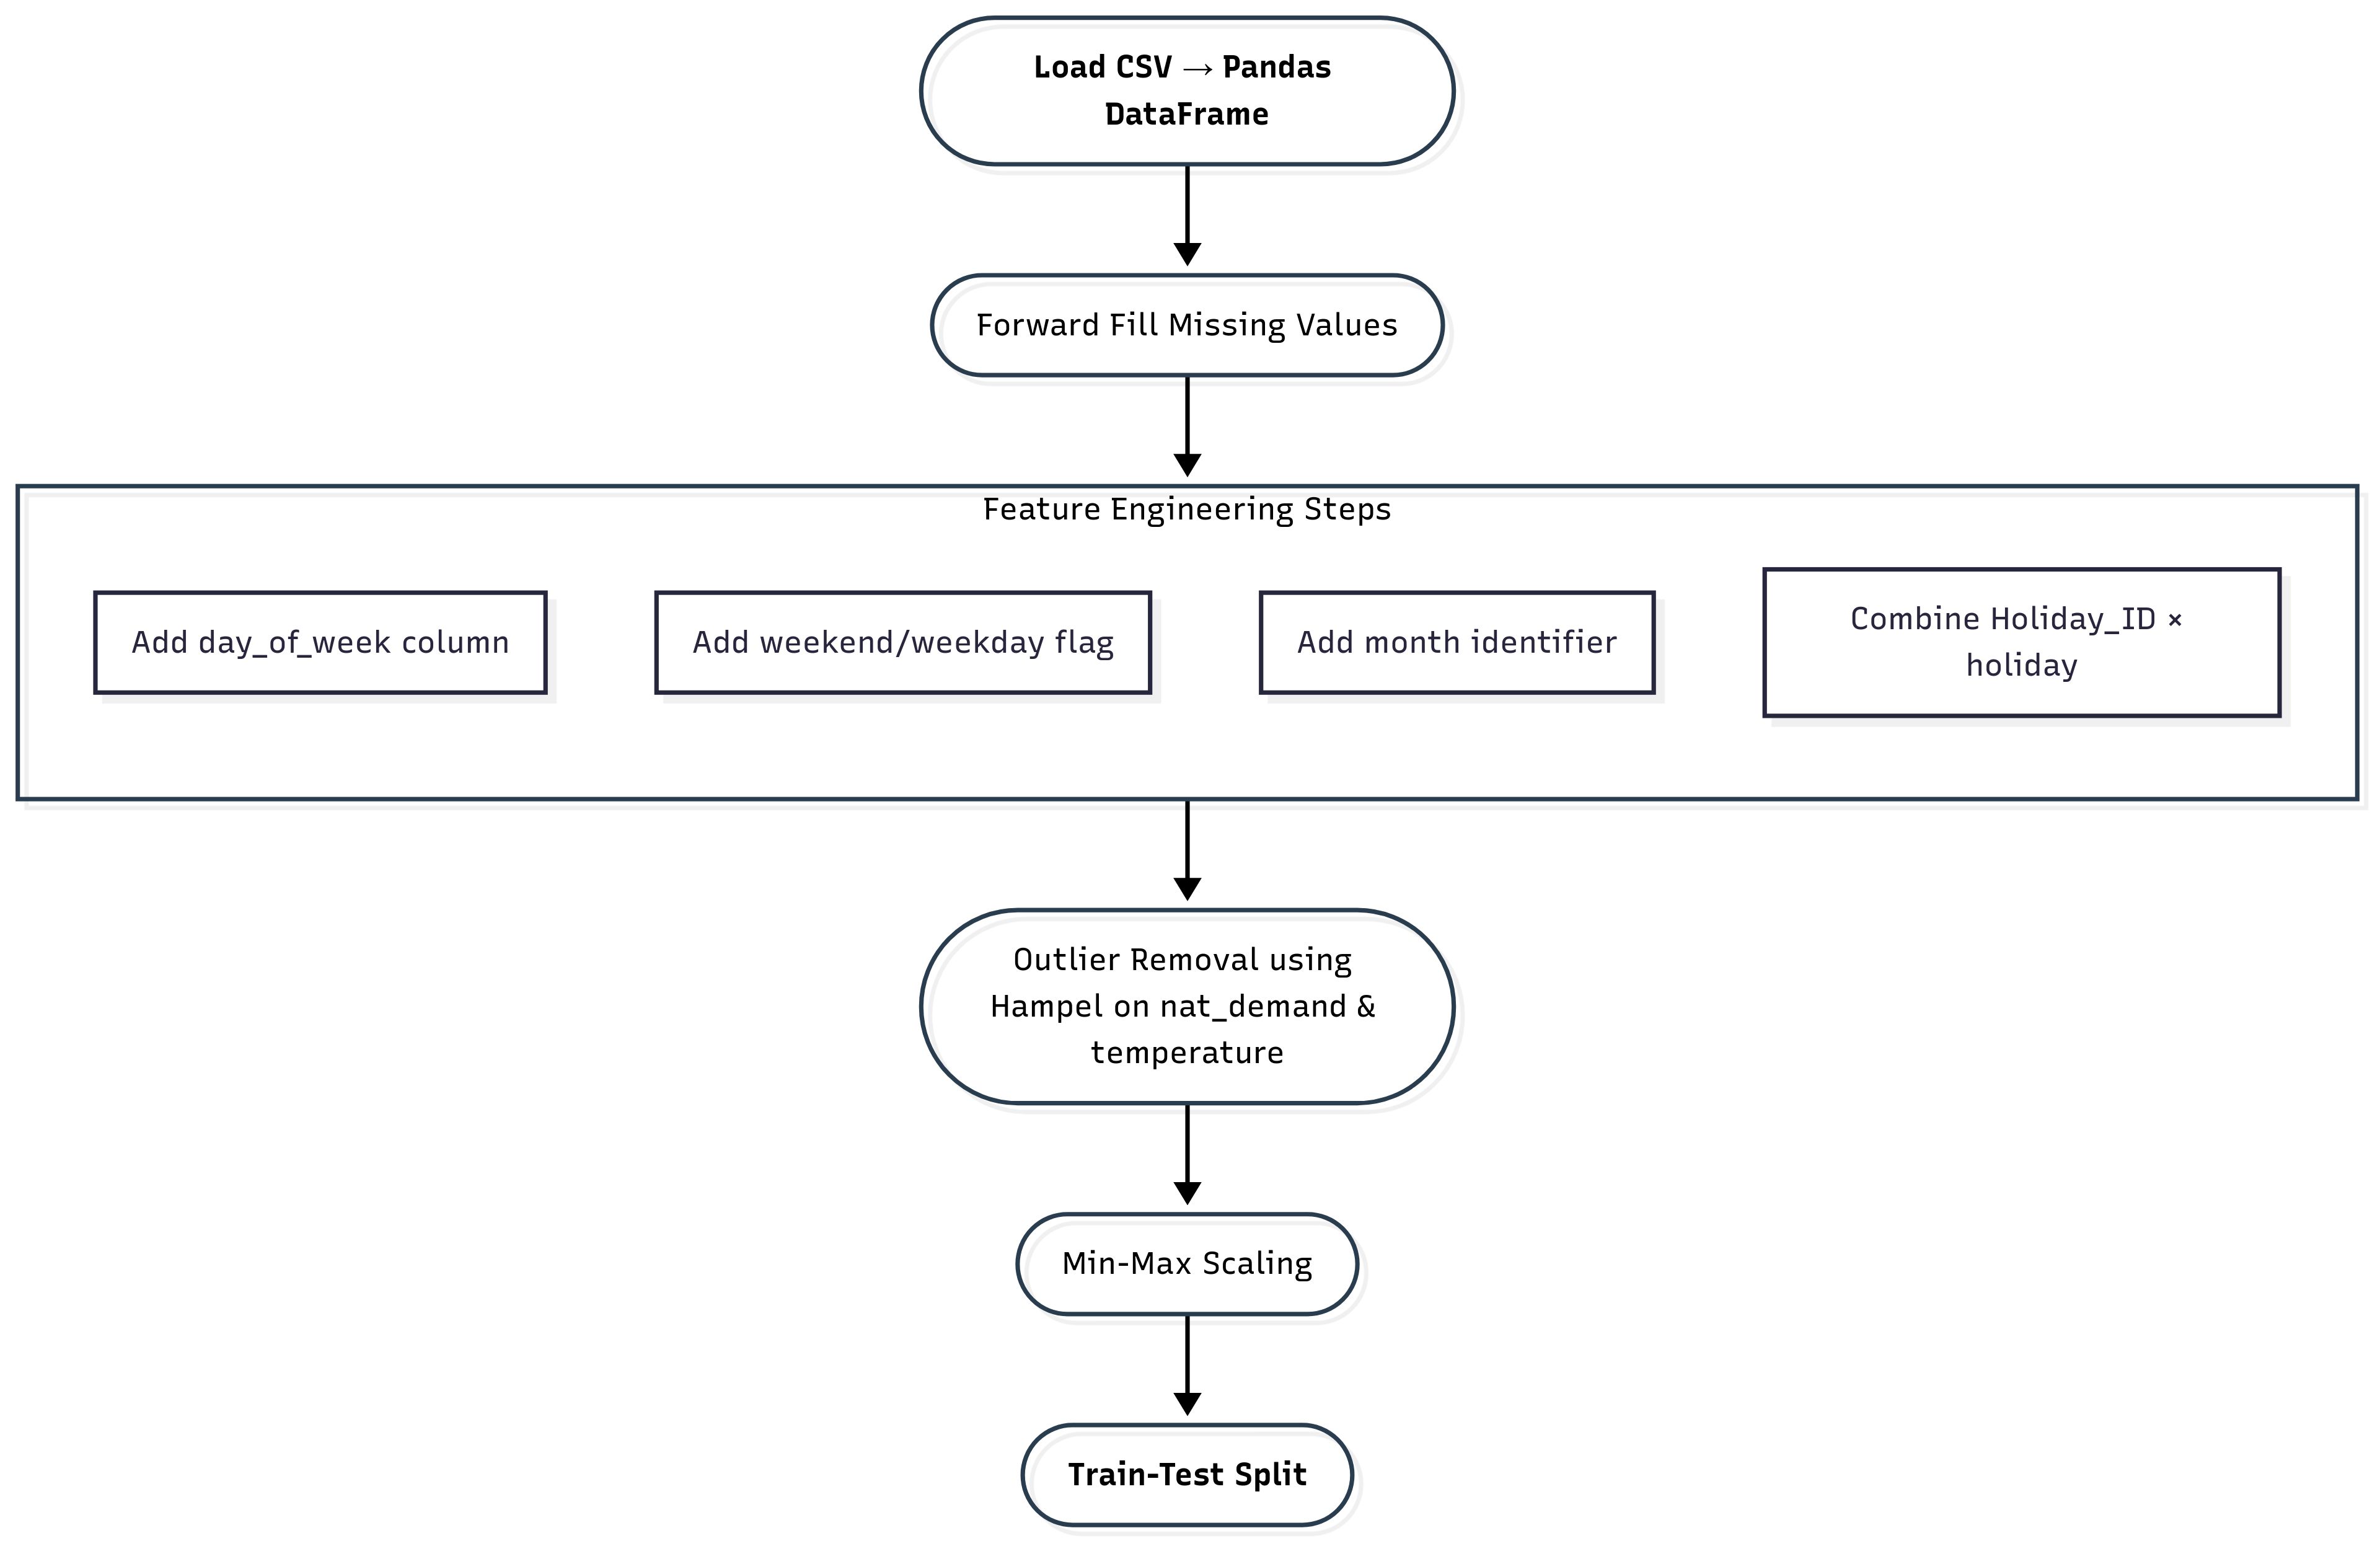
\includegraphics[width=0.7\linewidth]{Chapters/images/preprocess}
	\caption{The data preprocessing steps taken to process the data for model training}
	\label{fig:preprocessing}
\end{figure}

The steps taken for the data preprocessing are shown in the fig \ref{fig:preprocessing} 

\section{Evaluation Metrics}
The models were compared using standard error metrics and information criteria that are widely used in forecasting literature. These metrics provide complementary views on model performance in terms of accuracy, error magnitude, and model complexity. The chosen metrics are briefly described below. 

\subsubsection{Mean Absolute Percentage Error (MAPE)} 
MAPE expresses forecast accuracy as a percentage, making it easy to interpret across different scales. Lower values indicate better performance.  
\[
\text{MAPE} = \frac{100}{n}\sum_{t=1}^{n} \left| \frac{Y_t - \hat{Y}_t}{Y_t} \right|
\]

\subsubsection{Mean Squared Error (MSE)} 
MSE penalises larger errors more heavily by squaring them, making it sensitive to outliers.  
\[
\text{MSE} = \frac{1}{n}\sum_{t=1}^{n} (Y_t - \hat{Y}_t)^2
\]

\subsubsection{Root Mean Squared Error (RMSE)} 
RMSE is the square root of MSE and brings the error measure back to the same scale as the original data.  
\[
\text{RMSE} = \sqrt{\frac{1}{n}\sum_{t=1}^{n} (Y_t - \hat{Y}_t)^2}
\]

\subsubsection{Coefficient of Determination ($R^2$)} 
$R^2$ measures how well the forecasts explain the variance in the actual data. Higher values (closer to 1) indicate better fit.  
\[
R^2 = 1 - \frac{\sum_{t=1}^{n} (Y_t - \hat{Y}_t)^2}{\sum_{t=1}^{n} (Y_t - \bar{Y})^2}
\]

\subsubsection{Akaike Information Criterion (AIC)} 
AIC balances model fit and complexity. It penalizes over-parameterized models, with lower values indicating a better trade-off.  
\[
\text{AIC} = 2k - 2\ln(\hat{L})
\]
where $k$ is the number of model parameters and $\hat{L}$ is the maximized likelihood.



\section{Statistical and Machine Learning Models}
\subsection{Exponential Smoothing}

Exponential smoothing has been widely used as a method for STLF due to its low computational needs and fast processing times. The core idea of this method is to produce a forecast from an exponentially weighted average of past observations, giving the largest weight to the most recent data and exponentially decreasing weights to older data \cite{ostertagova2011simple}. This method's functionality has been discussed extensively in section \ref{sec:exponential smoothing}. In this section we will focus on the theoretical fundamentals and the choice of model we used in our research.  

There are multiple forms of ES, each designed to capture different components of a time series data.
\paragraph{Simple Exponential Smoothing(SES)}\label{par:ses}
SES is designed for time series datasets that lack seasonality and trend. The forecast is based solely on the weighted average of past observations. If $\hat{Y}_{t}$  is the value at time t  and $\alpha$ is the smoothing parameter between 0 and 1. The equation for the smoothed value $S_{t}$ would be \ref{eqn:6} as adapted from \cite{ostertagova2011simple}.

\[
\hat{S}_{t+1}  = \alpha Y_t + (1-\alpha)\hat{Y}_t
\tag{6}
\label{eqn:6}
\]
 Though the simplicity of SES is good for very low computational tasks it is not favorable for STLF due to the high level of accuracy required in forecasting and the trend and seasonality present in the data.
 
 \paragraph{Double Exponential Smoothing (DES)} method introduces capturing of trend in the time series data. This is in addition to the already existing level component in SES \ref{par:ses}. The equation of DES as adapted from \cite{nist_double_exp_smoothing} would be:
 \[
  S_t = \alpha Y_t + (1-\alpha)(S_{t-1} + b_{t-1})
  \tag{7}
 \label{eqn:7}
 \] 
 \[
  b_t = \gamma (S_t - S_{t-1}) + (1-\gamma) b_{t-1}
  \tag{8}
 \label{eqn:8}
 \]
 
 where $b_t$ would be the estimated trend or slope of the dataset and $\gamma$ would be the smoothing parameter for the trend  between 0 and 1. The data shows a clear flat trend over the long-term and seasonality every 24 hours with a fast rise and peak demand during midday shown in image \ref{fig:weeklydemand}. This 24 hour seasonality brings us to the third ES model which s the Triple Exponential Smoothing (TES). 
 \begin{figure}[h]
 	\centering
 	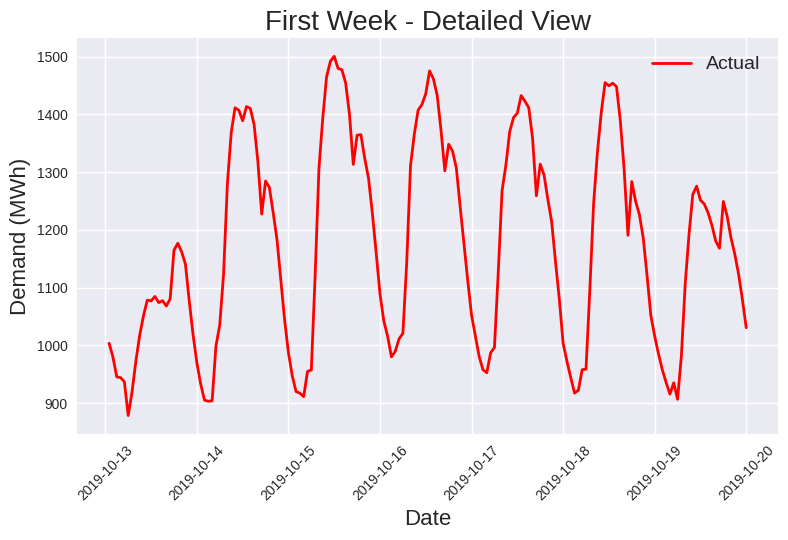
\includegraphics[width=0.7\linewidth]{Chapters/images/weekly_demand}
 	\caption{Real electricity demand from Sunday 13th to Saturday 20th of October 2019}
 	\label{fig:weeklydemand}
 \end{figure}
 
 \paragraph{Triple Exponential Smoothing } introduces the equation that takes care of the seasonality component of the data \cite{nist_double_exp_smoothing}. TES inherits equation \ref{eqn:7} and \ref{eqn:8} and introduces equation \ref{eqn:9} for seasonality adapted from \cite{nist_double_exp_smoothing}.
 \[
 I_t = \beta \frac{Y_t}{S_t} + (1-\beta) I_{t-m}  
 \tag{9}
 \label{eqn:9}
 \]
 $I_t$ is the estimated seasonal component and $\beta$ is the seasonality constant that is between 0 and 1. With the combination of equation \ref{eqn:6} , \ref{eqn:8}  and \ref{eqn:9} the overall smoothed value equation would be \ref{eqn:10}. 
 \[
 S_t = \alpha \frac{Y_t}{I_{t-L}} + (1-\alpha)(S_{t-1}+b_{t-1})
 \tag{10}
 \label{eqn:10}
 \]
 
 \paragraph{Damping} is a mechanism used to reduce or dampen the trend in forecasts over long horizons \cite{taylor2003exponential}. This method makes the forecast trend more conservative, preventing it from overshooting the actual data , which is a common issue in ES methods projecting a linear trend indefinitely in the future \cite{taylor2003exponential}. The equation below is for the smoothed value inclusive of the damping factor $\phi$ which is between 0 and 1, adapted from \cite{taylor2003exponential}. With equation \ref{eqn:11.a} being the additive in level and equation \ref{eqn:11.b} being the multiplicative in level.
 \[
 	S_t = \alpha \frac{Y_t}{I_{t-L}} + (1-\alpha)\bigl(S_{t-1} + \phi\, b_{t-1}) 
 \tag{11.a}
 \label{eqn:11.a}
 \]
 
 
 \[
 S_t = \alpha \frac{Y_t}{I_{t-L}} + (1-\alpha)\bigl(S_{t-1} \cdot b_{t-1}^{\,\phi}\bigr)
 \tag{11.b}
 \label{eqn:11.b}
 \]
 

 \subsubsection{Choice of best Exponential Smoothing model}
 The objective of the research is to improve STLF by using Ml and AI methods. ES as a statistical method would  be the benchmark for comparison of the ML models. However because of the different variations of ES an algorithm was  developed to help choose the best performing ES model to be used as the benchmark for the rest of the project. The models performance were compared on their MAPE, MAE, Mean Squared Error(MSE), RMSE and the AIC.
 
 This algorithm would create a model using statsmodel holtwinters \cite{statsmodels_expsmoothing_doc} and test its performance of forecasts on the dataset. Different model's performance would be compared to each other. Image \ref{fig:exponential-smoothing-model-choice} in appendix A shows a flow chart of how the algorithm functions. Table \ref{tab:es_model_selection} shows the different models that were tested to find the best model and their results.
 


\begin{table}[ht]
	\centering
	\resizebox{\textwidth}{!}{%
		\begin{tabular}{lccccccc}
			\hline \\
			\textbf{Model} & \textbf{Trend} & \textbf{Seasonality} & \textbf{Seasonality Period} & \textbf{Damped} & \textbf{MAPE (\%)} & \textbf{MSE (MWh)} & \textbf{AIC}
			 \\
			\hline
			Simple               & None  & None & –  & No  & 13.76\%  & 180.98 & 343990.96 \\
			Double               & Add   & None & –  & No  & 15.14\%  & 172.11 & 327001.68 \\
			Triple\_Add          & Add   & Add  & 24 & No  & 10.56\%  & 125.56 & 277981.02 \\
			Triple\_Mul          & Mul   & Mul  & 24 & No   & 34.48\%  & 408.23 & 272265.85 \\
			Triple\_Add\_Damped  & Add   & Add  & 24 & Yes &  9.99\%  & 120.81 & 277708.98 \\
			Triple\_Mul\_Damped  & Mul   & Mul  & 24 & Yes & 10.01\%  & 119.49 & 272266.18 \\
			\hline
		\end{tabular}%
	}
	\caption{Exponential Smoothing Models chosen for benchmarking and their performance.}
	\label{tab:es_model_selection}
\end{table}

Comparison of performance metrics through the algorithm in figure \ref{fig:exponential-smoothing-model-choice} was the Triple Multiplicative Damped algorithm with a seasonality period of 24 data points. Since the dataset is sampled hourly the seasonality was set to 24 hours. The MAPE and MSE are very close to each other with a difference of about 0.01 each. However the AIC value for  $Triple\_Mul\_Damped$ is lower than the one for $Triple\_Add\_Damped$, this showing a better model fit for  $Triple\_Mul\_Damped$. The final choice for the ES model was  $Triple\_Mul\_Damped$ and it served as a benchmark for testing performance of other models used in the experiment.
\subsubsection{Implementation of the Triple Multiplicative Damped ES model}



\subsection{Deep Belief Network}
 
 A DBN is a probabilistic generative model composed of multiple layers of stochastic, latent variables \cite{zhang2017deep}. It is constructed by stacking multiple layers of RBMs on top of each other \cite{zhang2016short}. This model benefits from its capabilities of limiting the occurrence of the local minima by pre-training RBMs using unsupervised training to adjust weights and parameters to ensure an enhanced performance in actual prediction use cases.
 
\subsubsection{Restricted Boltzmann Machine (RBM)}

A Restricted Boltzmann Machine (RBM) is a two-layer probabilistic generative model designed to learn the underlying probability distribution of input data. RBMs are widely used as building blocks for constructing DBNs \cite{dong2021short}. The architecture consists of a \textit{visible layer}, which receives the observed data, and a \textit{hidden layer}, which captures latent features and higher-order correlations in the data. Learning in RBMs is unsupervised: the model attempts to represent the structure of the input data by adjusting its parameters weights and biases so as to maximize the likelihood of the training samples \cite{zhang2017deep}.

An RBM is defined by a weight matrix that connects each visible unit to each hidden unit in a bipartite manner, together with bias vectors for both layers. No intra-layer connections are permitted, which simplifies inference and training. The structure is shown in figure \ref{fig:singlerbm}, adapted from Zhang et al. \cite{zhang2017deep}.

\begin{figure}[ht]
	\centering
	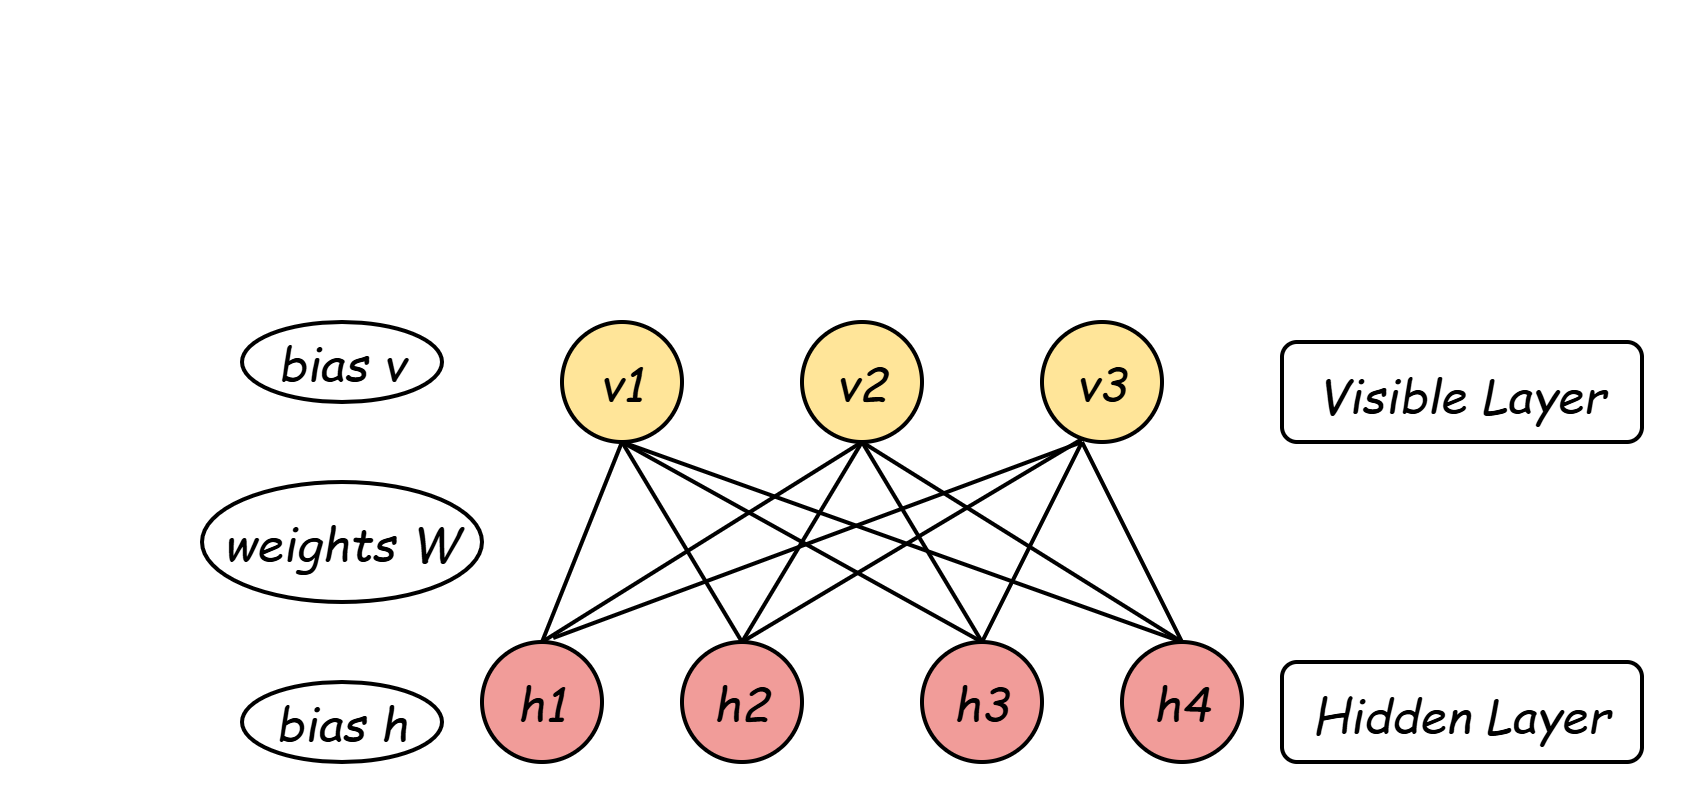
\includegraphics[width=0.7\linewidth]{Chapters/images/singleRBM}
	\caption{Illustration of an RBM with visible and hidden layers, including weights and biases}
	\label{fig:singlerbm}
\end{figure}

\paragraph{Energy-Based Formulation: } 
An RBM is an energy-based model, meaning it assigns a scalar energy value to each configuration of visible and hidden units. Configurations with lower energy are more likely under the model. The energy function is given by \cite{kong2019improved, zhang2016short}:

\[
E(v,h;\theta) = -\sum_i a_i v_i - \sum_j b_j h_j - \sum_{i,j} v_i W_{ij} h_j
\tag{12}
\label{eqn:12}
\]

where
\begin{itemize}
	\item $v_i$: the state of visible unit $i$,
	\item $h_j$: the state of hidden unit $j$,
	\item $a_i$: the bias associated with visible unit $i$,
	\item $b_j$: the bias associated with hidden unit $j$,
	\item $W_{ij}$: the weight between visible unit $i$ and hidden unit $j$,
	\item $\theta = \{W, a, b\}$: the model parameters.
\end{itemize}

\paragraph{Probability Distribution: } 
Using the energy function, the joint probability of a visible–hidden configuration is defined by the Boltzmann distribution \cite{DBN_GeeksforGeeks}:

\[
P(v,h) = \frac{e^{-E(v,h)}}{Z}
\tag{13}
\label{eqn:13}
\]

where $Z$ is the \textit{partition function}, given by summing over all possible visible and hidden states:
\[
Z = \sum_{v,h} e^{-E(v,h)}
\]

The probability of a visible vector $v$ is obtained by marginalizing out the hidden layer:
\[
P(v) = \frac{1}{Z} \sum_{h} e^{-E(v,h)}
\]

\paragraph{Training RBMs:} 
RBMs are typically trained using the \textit{Contrastive Divergence} (CD) algorithm. Training consists of two phases:

\begin{enumerate}
	\item \textbf{Positive phase:} a visible vector from the data activates the hidden layer, and correlations $\langle v_i h_j \rangle_{\text{data}}$ are computed.
	\item \textbf{Negative phase:} the hidden units are used to reconstruct the visible layer, producing a reconstructed vector. From this, correlations $\langle v_i h_j \rangle_{\text{recon}}$ are obtained.
\end{enumerate}

The difference between the two phases provides the learning signal for updating weights:
\[
\Delta W_{ij} = \eta \Big( \langle v_i h_j \rangle_{\text{data}} - \langle v_i h_j \rangle_{\text{recon}} \Big)
\tag{14}
\label{eqn:14}
\]
where $\eta$ is the learning rate. In this way, the RBM iteratively learns to reduce the gap between the distribution of the training data and the distribution it models. The feed-forward (data-to-hidden) and feed-backward (hidden-to-reconstruction) passes, together with weight updates, constitute the CD training loop \cite{RBM_GeeksforGeeks}.

\paragraph{RBMs are stacked to create a DBN} When 1 or more RBMs are stacked together they create a DBN. This DBN has the advantage of pre-trained RBMs that have adjusted their weightings to minimize error in the training phase. Stacking of RBMs is as shown in the figure \ref{fig:correctrbm}.
\begin{figure}[h]
	\centering
	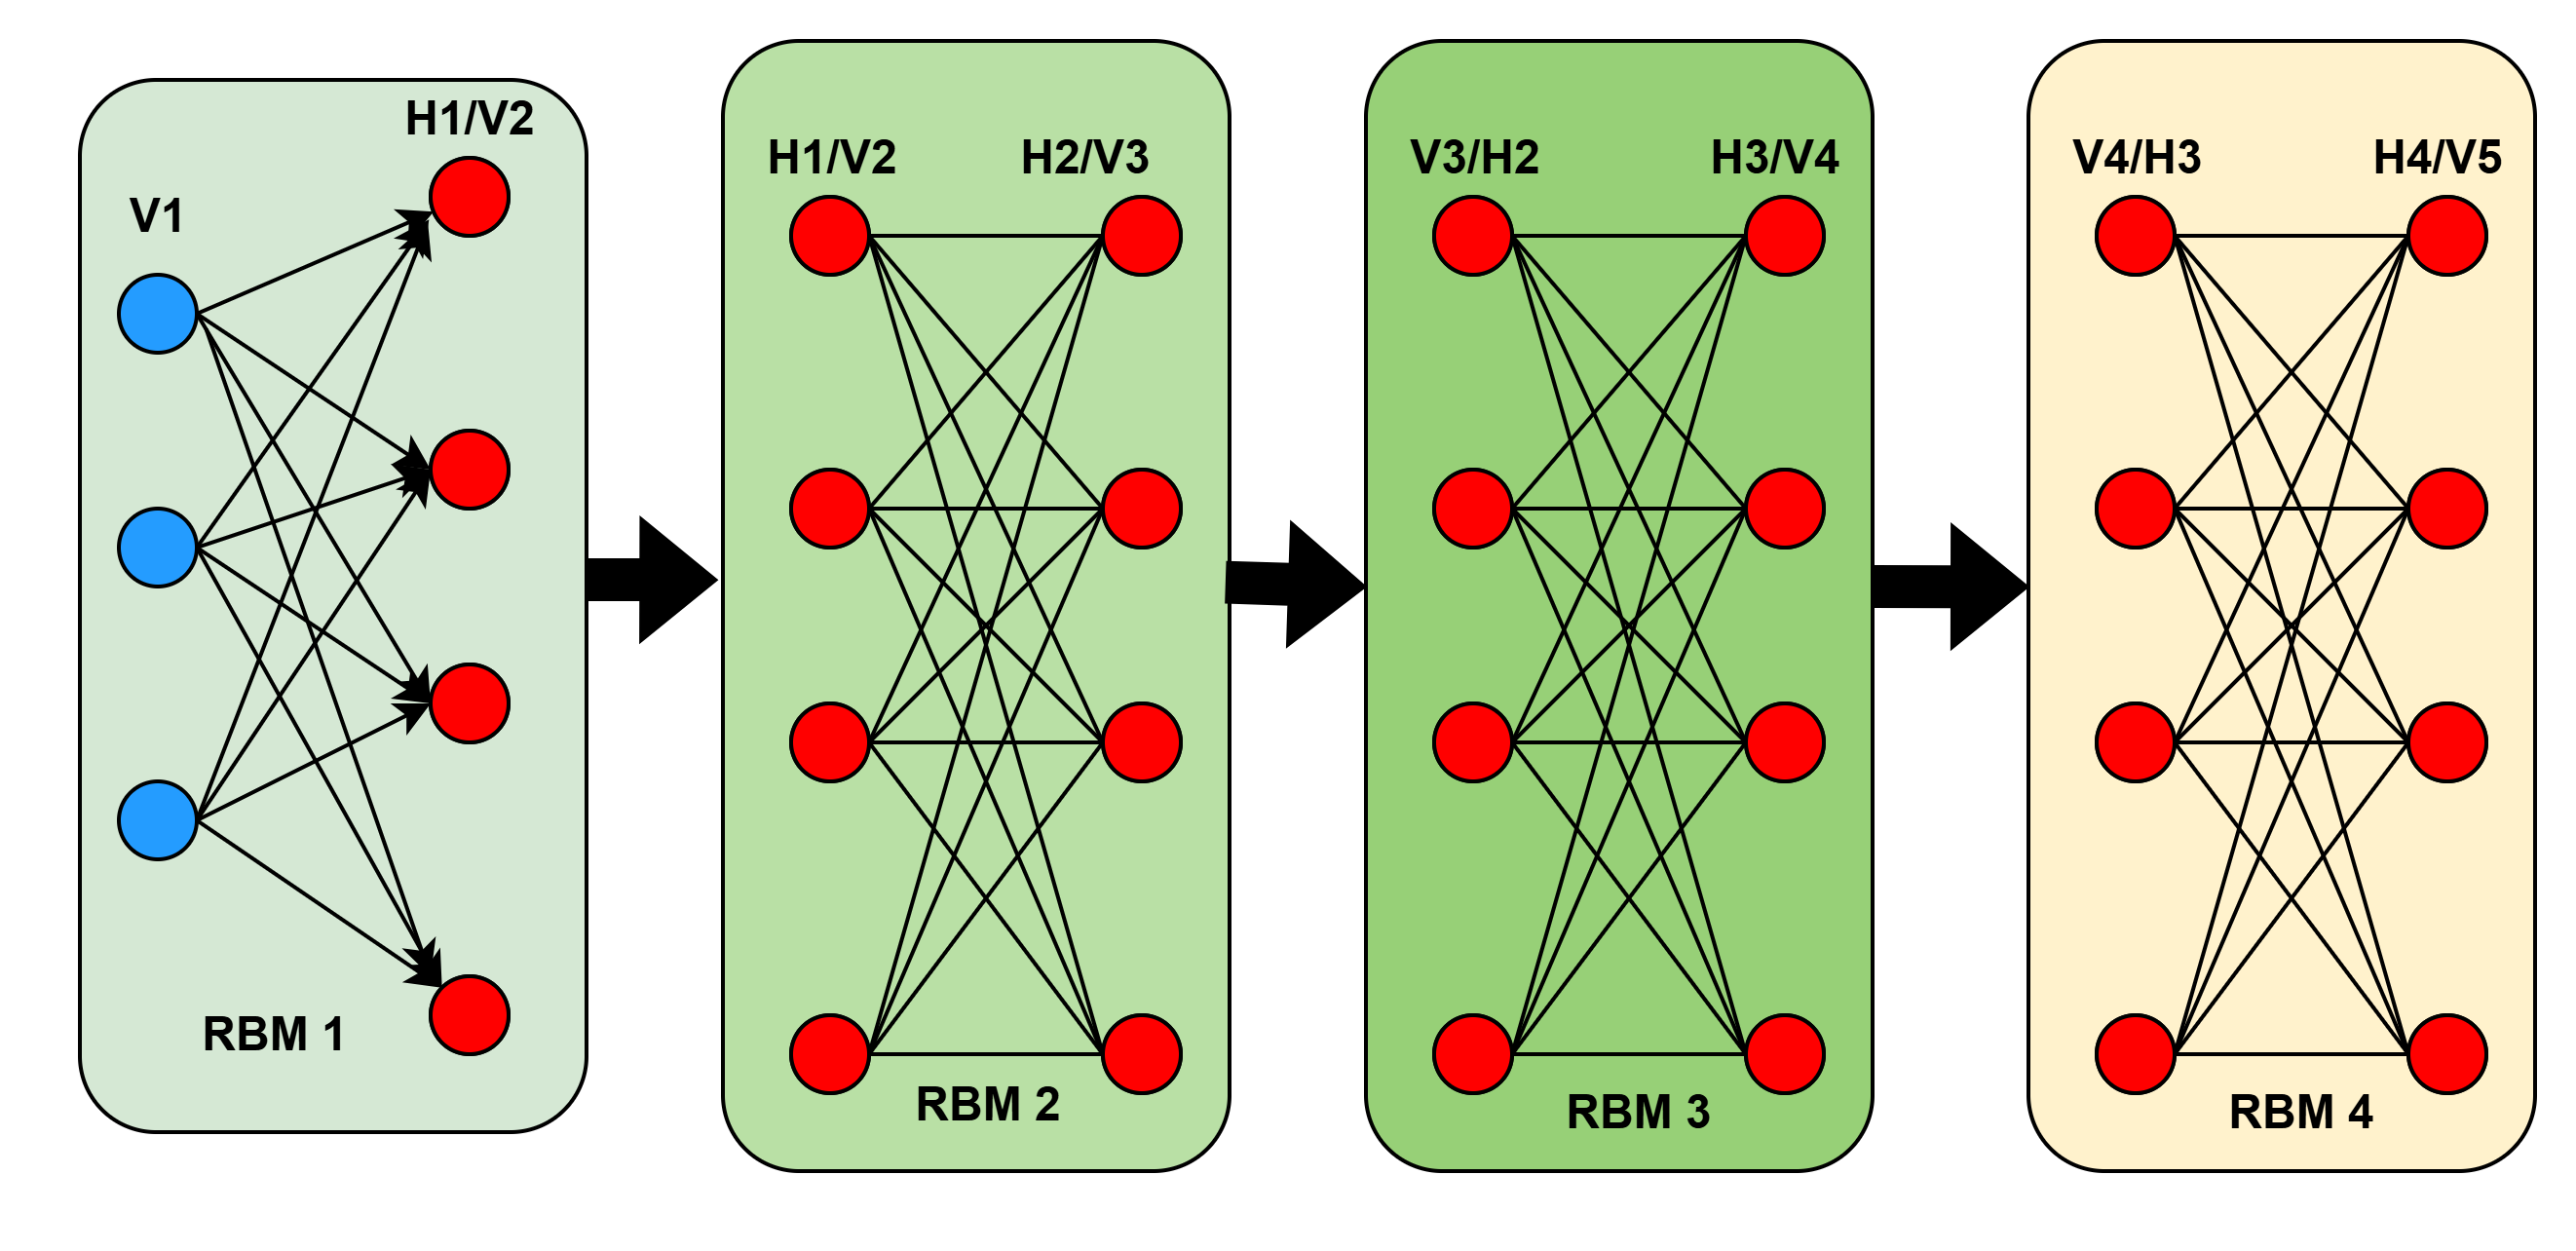
\includegraphics[width=0.7\linewidth]{Chapters/images/CORRECT_RBM}
	\caption{An illustration of stacked RBMs making a DBN}
	\label{fig:correctrbm}
\end{figure} 
This illustration highlights how the hidden layer of the first RBM is the visible layer of RBM 2. During pretraining each RBM is trained separately RBM1 will receive the original data and perform CD on RBM1, the recreated output on the hidden layer 1(HD1) becomes the input of RBM2 through the visible layer 2(V2). RBM2 will go through CD and continues the loop until the full RBM has been trained.

\subsection{Implementation of DBN architecture for STLF}
The proposed DBN designed for the STLF task, leverages its hierarchical feature extraction capabilities to model complex temporal and non linear dependencies present in the time series data.

The DBN was implemented using \textit{tensorflow.keras.callbacks} for fitting, evaluating and prediction functionality of the model. The DBN also uses \textit{tensorflow.keras.layers} for creating the different RBM layers in the model. Scikit-learn was also used for data scaling and evaluating performance using features such as the \textit{MinMaxScaler} and \textit{mean\_absolute\_percentage\_error}. 
\subsubsection{Input Feature Engineering}
The original dataset went through its initial feature engineering as explained in section \ref{sec:datapreprocessing}, however further feature engineering is performed to enhance performance.

\begin{enumerate}
	\item \textbf{Lagged Load Values : } This is essential for capturing time series auto correlation, to do so the network uses lagged values of nat\_demand at $\tau$ = [1,2,3,7,24,168] hours . These lags will enable capturing past demand for 1-3 hours, 24 hours and 168 hours which is a week. The lags are important for capturing seasonality and aligns with the seasonality benchmark in the ES implementation.
	\item \textbf{Cyclical Encoding : } To avoid discontinuities and ensure the network learns smooth transition of time eg from 11PM to 12 AM , cyclical encoding is applied to hour, day of week and month. With cyclical encoding the times 11PM and 12AM are represented as being close to each. This is performed by using sine and cosine transformation to the dataset columns associated.
	\item \textbf{Rolling Statistics : } Mean and standard deviation of nat\_demand over 7 and 24-hour windows are included to capture recent trend and volatility.
\end{enumerate}
All missing values resulting from lag and rolling window operations were handled through forward and backward filling, followed by complete case removal to ensure data integrity. The final feature set comprised approximately 20-25 input variables depending on the available data columns.
\subsubsection{DBN Structure}
The DBN structure comprises a stacking of 3 RBMs, forming a deep architecture representation. Table \ref{tab:dbn_architecture} shows the representation of each layer.
\begin{table}[h]
	\centering
	
	
	\resizebox{\textwidth}{!}{%
	\begin{tabular}{lccc}
		\hline \\
		\textbf{Layer Type} & \textbf{Units ($\boldsymbol{n}_{\mathbf{h}}$)} & \textbf{Activation (RBM Pre-training)} & \textbf{Activation (Fine-Tuning)} \\
		\hline
		\\
		RBM 1 (H1) & 256 & Sigmoid ($\sigma$) & ReLU \\
	
		RBM 2 (H2) & 128 & Sigmoid ($\sigma$) & ReLU \\
	
		RBM 3 (H3) & 64 & Sigmoid ($\sigma$) & ReLU \\
	
		Fine-Tuning Layer & 32 & N/A & ReLU \\
	
		Output Layer & 1 & - & Linear (None) \\
	\hline
	\end{tabular}
}
	\caption{DBN Layer configuration}
	\label{tab:dbn_architecture}
\end{table}

The architecture had 3 RBMs setup with 256, 128 and 64 units respectively. Each of these layers were trained using CD , before being stacked and initialized for the deep network. The final layer added a dense layer of 32 ReLU units for fine=tuning and a linear regression output layer for predicting continuous load values. The ReLu activation function is chosen due to its ability to mitigate to the disappearing gradient problem \cite{bibid}.\\
 The fine tuning layer acts as the combiner of RBM-initialized layers, putting them together before the output layer. This design implementation was chosen to allow the network to learn task specific transformations on top of the general features learned during unsupervised learning.\\ The final output layer is a single dense linear unit without an activation function, producing a continuous regression output representing the forecasted electricity demand. This type of output is appropriate for regression tasks as it allows the network to predict values across the full range of the target value without constraints.
\textbf{ADD AN IMAGE OF THE DBN}

\subsection{Training Procedure}
 DBN training is split into two sections, unsupervised learning for the RBMs and supervised learning for the stacked RBMs. These procedures will effectively initialize a deep forward netowrk to a good starting point.
 \subsubsection{Pre-training (Unsupuervised)}Each of the RBMs are trained sequentially using the input data X\_train is an unsupervised manner to learn a robust and hierarchical representation of the input features. The CD algorithmn explained in \ref{label} is what is used to train each RBM, approximating the gradient using the error equation \ref{}. A fixed momentum term of 0.9 is set to accelerate convergence and dampen oscillation.\\ The learning rate was implemented during the pretraining, starting at 0.01 for the first layer and decaying by a factor or 0.8 for each subsequent RBM layer. This decaying factor is to counter the increasing abstraction in higher layer which will require the updates of the layers to be more conservative. Each RBM is trained for 25 epochs, this is because there was a negligible change in the final prediction with increased epochs.
 
 \subsubsection{Fine-Tuning (Supervised)} Following the supervised pre-training, the network was unrolled nto a standard feed-forward neural network and fine tuned using supervised learning. The learned RBM weights and biases from the pre-training are transferred to initialize the corresponding dense layers in the supervised network. This initialization provides the network with meaningful feature representation. After the transfer the network will learn through supervised learning using standard back-propagation method which will train the network end-to-end.
 The Adam optimizer is chosen with a base learning rate of 0.001. Adam is preferred over standard SGD for deep learning due to its adaptive learning rates for individual parameters, leading to faster and more stable convergence. The network is then compiled using MSE as its loss function, which is appropriate for regression tasks and is minimized during training.
 
 \subsubsection{Regularization Strategies}
 Multiple regularization strategies were employed to prevent overfitting and improve generalization.
 
 \begin{itemize}
 	\item \textbf{L2 Weight Decay} : Applied to the kernel weights of all dense layers with a factor of 0.001 to prevent overfitting by penalizing large weights.
 	\item \textbf{Dropout} : A dropout rate of 0.2 is applied between the hidden layers, and a lower rate (0.1) is applied to the input layer and the final fine-tuning layer to prevent over-reliance on specific neurons.
 	\item \textbf{Early Stopping} : Training terminates if the validation loss) does not improve for 15 consecutive epochs. The best weights corresponding to the lowest validation loss are restored.
 	\item \textbf{Reduce LR On Plateau} : The learning rate is dynamically halved (factor=0.5) if the validation loss plateaus for 8 epochs, ensuring the model can escape local minima.
 \end{itemize}
 
 \textbf{ ADD AN IMAGE OF THE COMPLETE STEP BY STEP OF THE INITIALIZATION AND TRAINING OF THE DBN}
 
 
 The DBN was evaluated using three complementary metrics to capture the different aspects of forecasting accuracy. MAPE, MAE and RMSE were used to evaluate and compare the DBN with the other models. These evaluations were performed on inverse transformed predictions to ensure the validation occurred in the original load scale rather than the normalized space used for training. Performance was also assessed separately on both training and test sets to monitor potential overfitting and evaluate generalization capability.
 
 
 
 \subsection{Long Short Term Memory}
		\chapter{Results}
In this section we present and compare results of the four models aplied in STLF. The performance of the models are evaluated using MAPE, MAE, RMSE and R\^2. These metrics can give us a clear picture and comparisons framework for each of the model performance.  The goal is to represent the accuracy, robustness and suitability of the ML and AI models to solve STLF.

The metrics theory is explained in \ref{sec:eval_metrics} which shows the mathematics behind each of the metrics used in the research. The methodology shows the creation of the models and how these results were produced. 


\section{Dataset Results}
 The continuous\_dataset.csv contained well ordered data that was collected with minimum errors, empty data was filled using the forward and back-filling process.Figure \ref{fig:originaldataset}
 \begin{figure}[h]
 	\centering
 \begin{minipage}[b]{0.45\linewidth}
 	\centering
 	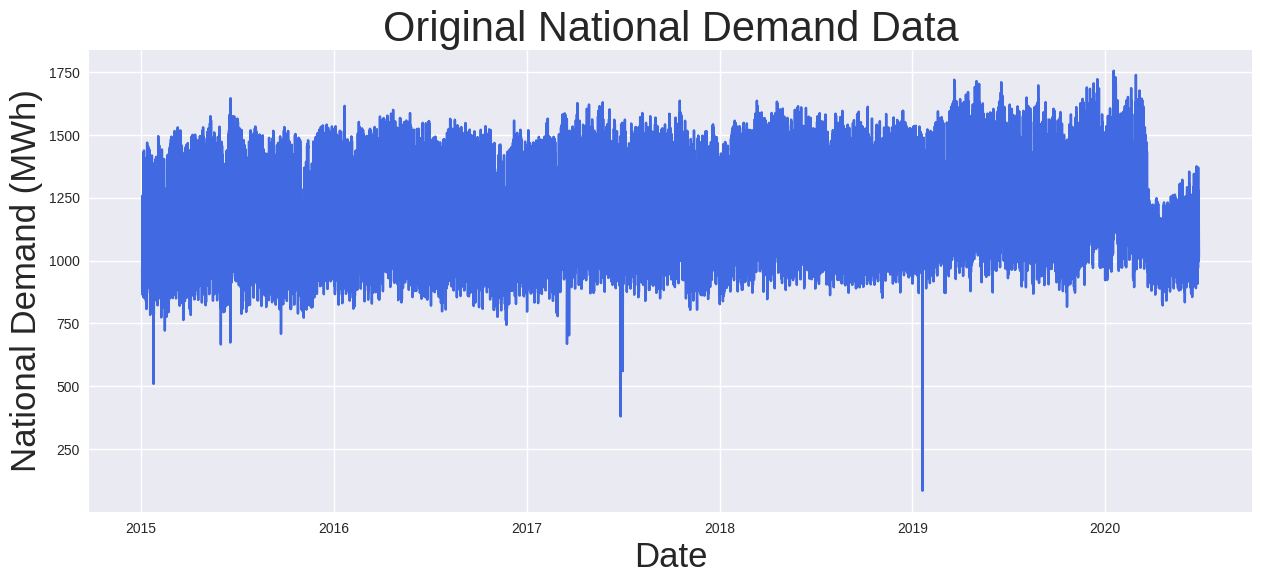
\includegraphics[width=\linewidth]{Chapters/images/results/original_dataset}
 	\caption{The original national demand .}
 	\label{fig:originaldataset}
 \end{minipage}
 \begin{minipage}[b]{0.45\linewidth}
 	\centering
 	\includegraphics[width=\linewidth]{"Chapters/images/results/train test split_after HI"}
 	\caption{HI processed dataset with traintest split.}
 	\label{fig:train-test-splitafter-hi}
 \end{minipage}
 \end{figure}
 
 The HI method explained in section \ref{sec:HI_method}, was used to handle outliers in the dataset, fixing all data-points that deviated from the normalcy presented in the dataset. After the implementation of the HI-method the train test split of 80/20 was implemented. Figure \ref{fig:train-test-splitafter-hi} shows the effectiveness of the HI method in removing noisy details in the dataset.

 \begin{figure}[h]
  	\centering
  	% First figure
  	\begin{minipage}[b]{0.45\linewidth}
  		\centering
  		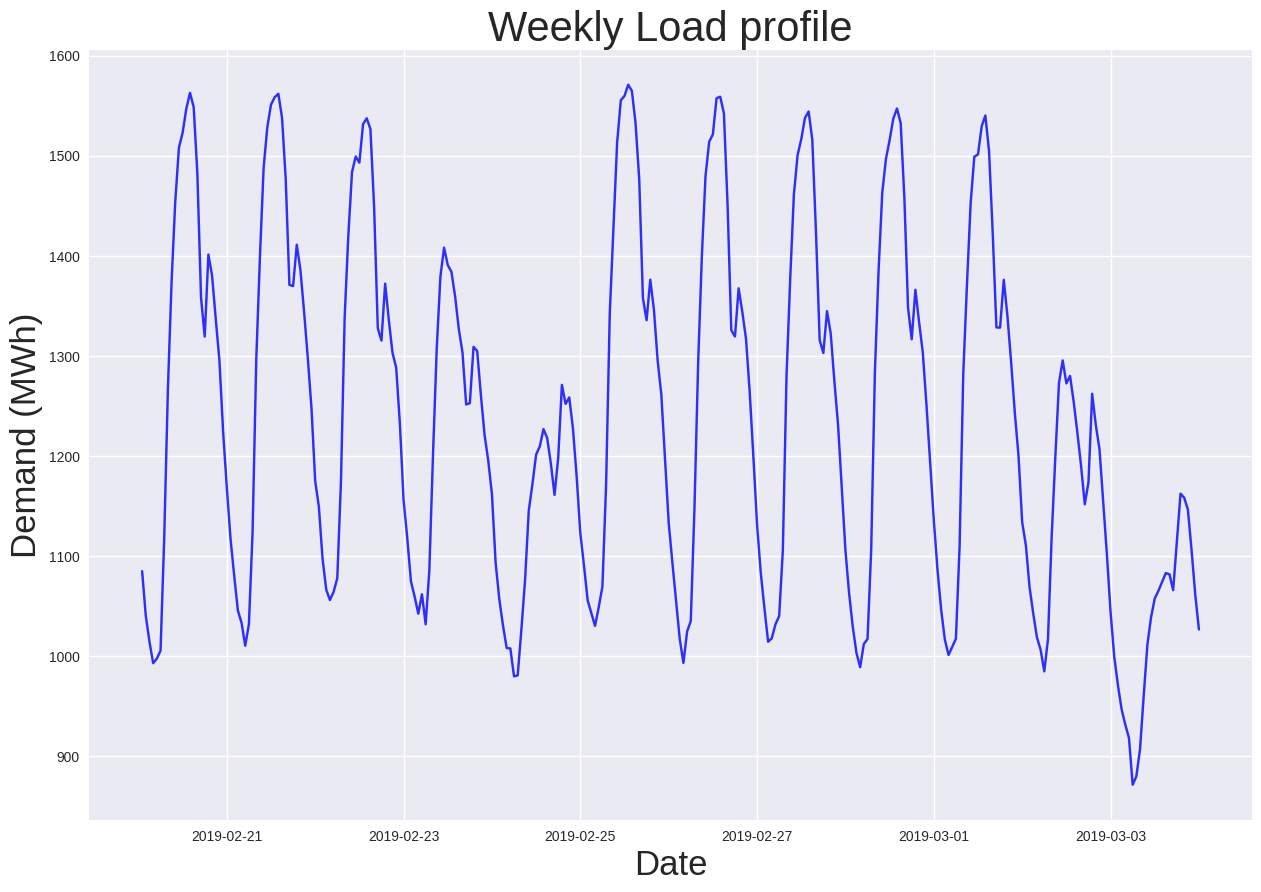
\includegraphics[width=\linewidth]{Chapters/images/results/weekly_load_profile.png}
  		\caption{The general weekly national load profile.}
  		\label{fig:weeklyloadprofile}
  	\end{minipage}
  	\hfill
  	% Second figure
  	\begin{minipage}[b]{0.45\linewidth}
  		\centering
  		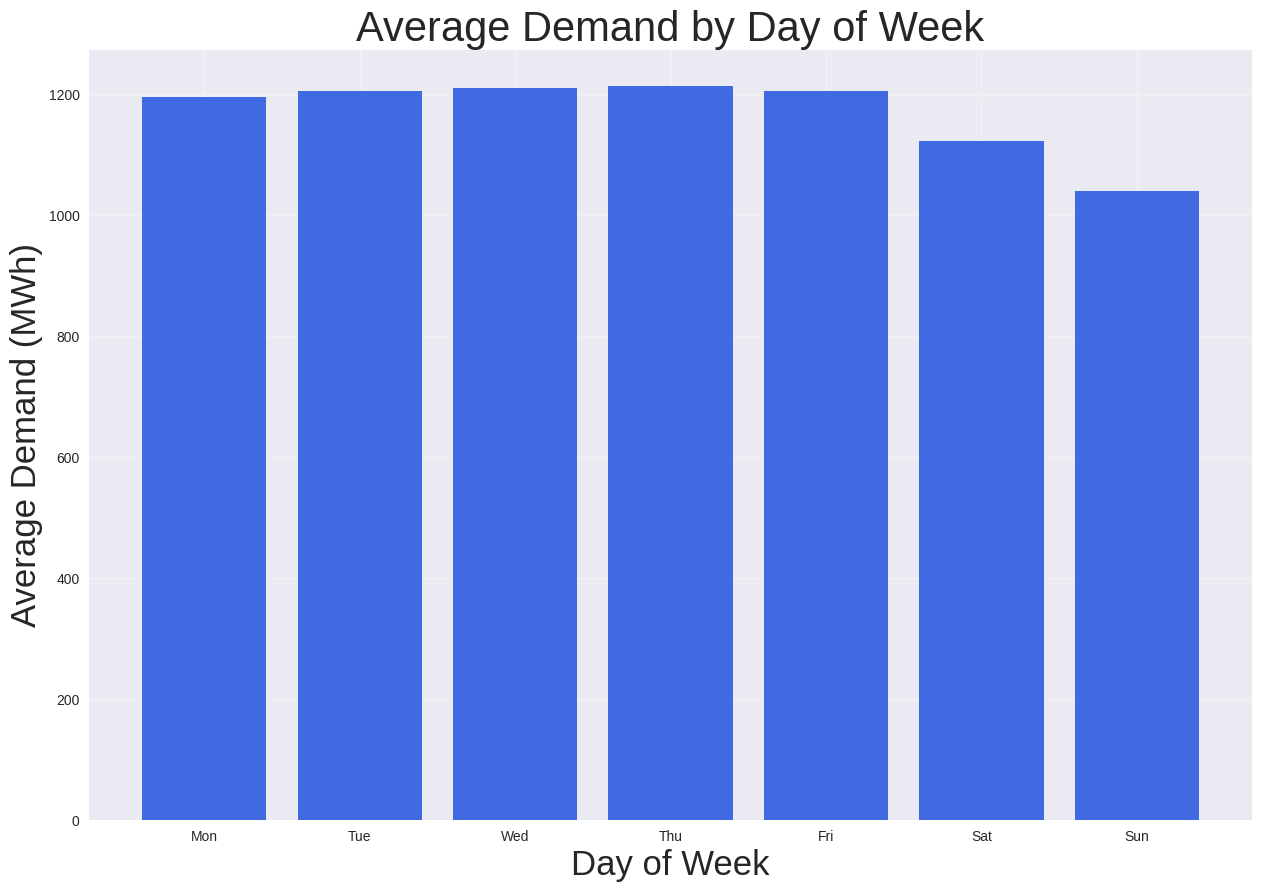
\includegraphics[width=\linewidth]{Chapters/images/results/average_daily_demand.png}
  		\caption{The weekly average daily demand }
  		\label{fig:averagedailydemand}
  	\end{minipage}
  \end{figure}
  
  
  To further understand the dataset, it was broken down to give the more insight on how the data and load behaves at different points. Firstly the weekly load profile in figure \ref{fig:weeklyloadprofile} shows a daily pattern that the load exhibits.The trend shows a higher usage during the week and lower usage in the weekend, with the lowest usage day being Sunday. 
  
  
  Figure \ref{fig:averagedailydemand} shows the average daily demand  of electricity. It also shows a higher usage during the week and lower consumption on the weekend, with Sunday being the lowest consumption day. 
  \begin{figure}[h]
  	\centering
  	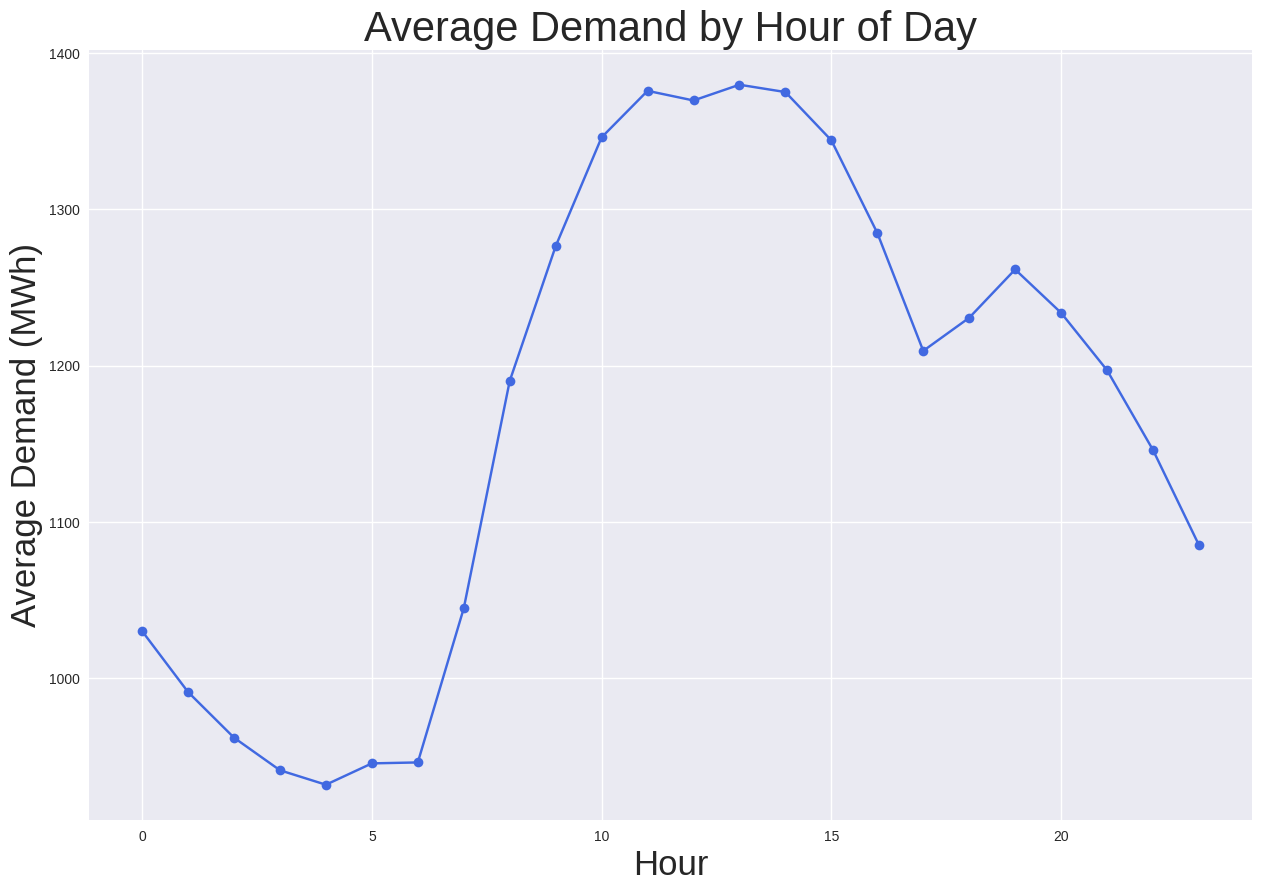
\includegraphics[width=0.45\linewidth]{Chapters/images/results/average_hourly_demand}
  	\caption{Average hourly demand of electricity between 2015 and 2020 in panama}
  	\label{fig:averagehourlydemand}
  \end{figure}
  
  Figure \ref{fig:averagehourlydemand} shows the average hourly usage of data. The averages show that the lowest consumption is in the early hours of the day, with a steady rise in the early morning leading to a peak at midday. After midday there is a steady decrease in demand with a slight increase between the 18th and 20th hour of the day, this is followed by a drop in usage leading to the early hours of the day.  


\section{Model Simulation Results}

\subsection{Exponential smoothing}
\subsubsection{Model Choice result}
The algorithm in  Appendix \ref{sec:appendixA} figure \ref{fig:exponential-smoothing-model-choice} was used to find the best model to use for the ES model.Table \ref{tab:es_model_selection} shows the different models that were tested to find the best model.

\begin{table}[ht]
	\centering
	\resizebox{\textwidth}{!}{%
		\begin{tabular}{lccccccc}
			\hline \\
			\textbf{Model} & \textbf{Trend} & \textbf{Seasonality} & \textbf{Seasonality Period} & \textbf{Damped} & \textbf{MAPE (\%)} & \textbf{MSE (MWh)} & \textbf{AIC}
			\\
			\hline
			Simple               & None  & None & –  & No  & 13.76\%  & 180.98 & 343990.96 \\
			Double               & Add   & None & –  & No  & 15.14\%  & 172.11 & 327001.68 \\
			Triple\_Add          & Add   & Add  & 24 & No  & 10.56\%  & 125.56 & 277981.02 \\
			Triple\_Mul          & Mul   & Mul  & 24 & No   & 34.48\%  & 408.23 & 272265.85 \\
			Triple\_Add\_Damped  & Add   & Add  & 24 & Yes &  9.99\%  & 120.81 & 277708.98 \\
			Triple\_Mul\_Damped  & Mul   & Mul  & 24 & Yes & 10.01\%  & 119.49 & 272266.18 \\
			\hline
		\end{tabular}%
	}
	\caption{Exponential Smoothing Models chosen for benchmarking and their performance.}
	\label{tab:es_model_selection}
\end{table}

Comparison of performance metrics through the algorithm in figure \ref{fig:exponential-smoothing-model-choice} was the Triple Multiplicative Damped algorithm with a seasonality period of 24 data points. Since the dataset is sampled hourly the seasonality was set to 24 hours. The MAPE and MSE are very close to each other with a difference of about 0.01 each. However the AIC value for  $Triple\_Mul\_Damped$ is lower than the one for $Triple\_Add\_Damped$, this showing a better model fit for  $Triple\_Mul\_Damped$. The final choice for the ES model was  $Triple\_Mul\_Damped$ and it served as a benchmark for testing performance of other models used in the experiment.
The models tested in the research were created using python and tensorflow, using google collab an cloud jupyter notebook environment for faster processing and version control through google drive. 

The ES model being the benchmark model achieved a MAPE of 9.57\% with a MAE of 118.18Mwh using the triple Multiplicative Damped model. Table \ref{tab:exp_smoothing_results} below contains the the results produced by the ES model and the parameters of the model. 
\begin{table}[h]
	\centering
	
	\begin{tabular}{ll}
		\hline
		\textbf{Metric / Parameter} & \textbf{Value} \\
		\hline
		\multicolumn{2}{l}{\textbf{Model Results}} \\
		AIC & 20118.40 \\
		MAPE &  9.57\% \\
		MAE & 118.14 \\
		RMSE & 141.84 \\
		Correlation & 0.7239\\
		\hline
		\multicolumn{2}{l}{\textbf{Model Parameters}} \\
		Smoothing Level ($\alpha$) & 1.0000 \\
		Smoothing Trend ($\beta$) & 0.0000 \\
		Smoothing Seasonal ($\gamma$) & 0.0000 \\
		Damping Trend ($\phi$) & 0.9744 \\
		Initial Level ($l_0$) & 1071.1459 \\
		Initial Trend ($b_0$) & 1.0236 \\
		Initial Seasons & [0.9093, 0.8828, 0.8638, 0.8555, 0.8682, ...] (shape = 24) \\
		Use Box-Cox & 0.0000 \\
		Lambda ($\lambda$) & None \\
		Remove Bias & 0.0000 \\
		\hline
	\end{tabular}
	\caption{Triple Multiplicative Damped Exponential Smoothing Model Parameters and Results}
	\label{tab:exp_smoothing_results}
\end{table}
These parameters produced the best results in comparison to other ES models and this was evaluated through the algorithm shown in  \ref{fig:exponential-smoothing-model-choice}. 
\begin{figure}[h]
	\begin{minipage}[b]{0.45\linewidth}
	\centering
	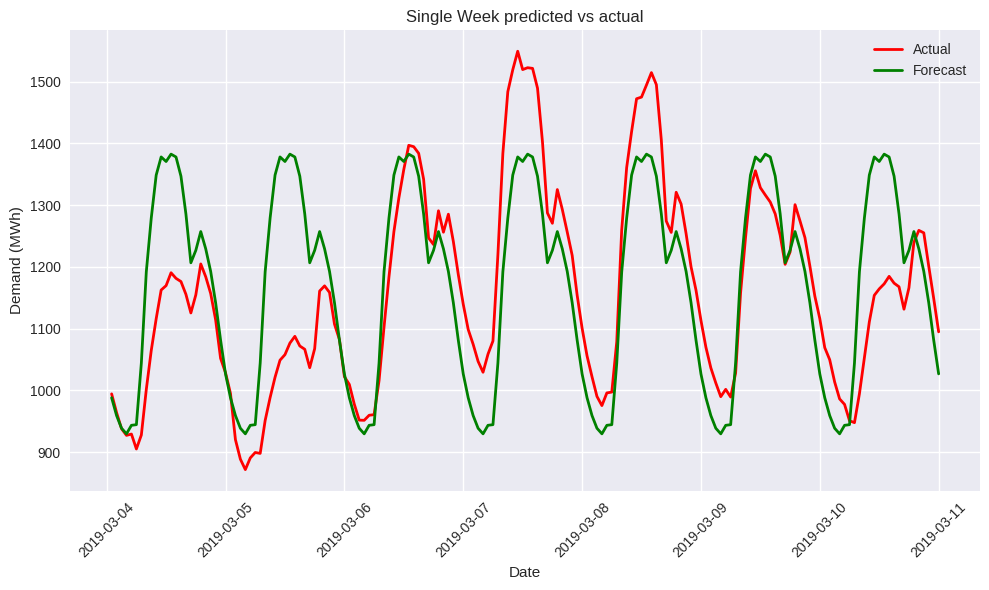
\includegraphics[width=\linewidth]{Chapters/images/results/ES_predicted_vs_actual}
	\caption{The ES predicted results against the actual demand in a week}
	\label{fig:espredictedvsactual}
\end{minipage}
\hfill
% Second figure
\begin{minipage}[b]{0.45\linewidth}
	\centering
	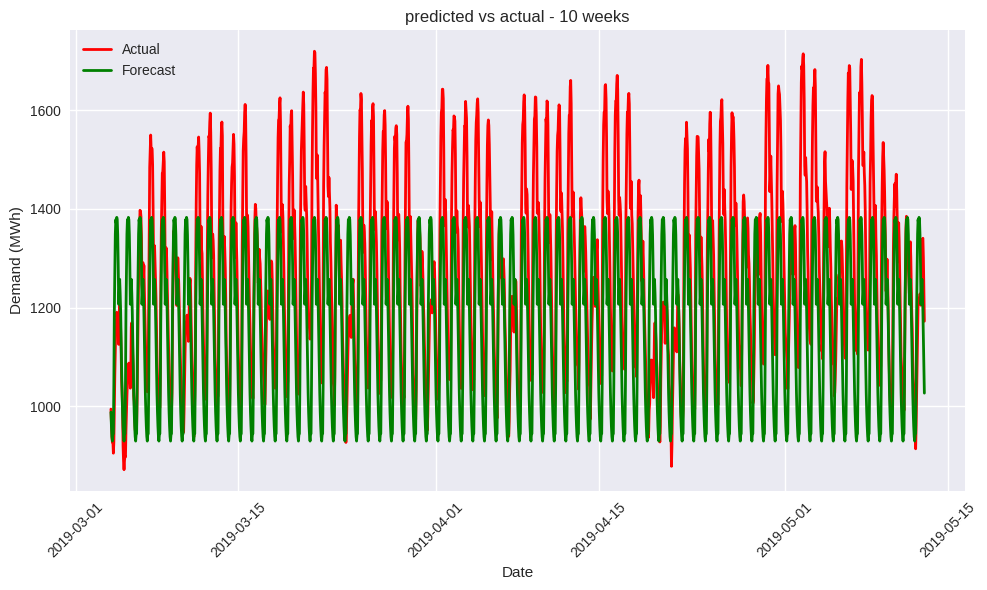
\includegraphics[width=\linewidth]{Chapters/images/results/ES_predicted_vs_actual_10weeks}
	\caption{ES model predicted vs actual load demand over 10 weeks}
	\label{fig:espredictedvsactual10weeks}
	
\end{minipage}
\end{figure}
 Figure \ref{fig:espredictedvsactual} shows the predicted and the actual values. This image shows that the model has learned the train data and does not adjust the prediction to the changing features.Figure \ref{fig:espredictedvsactual10weeks} further shows the generalization by the model. This is because ES models are not best suit for non linear problem sets.

\subsection{LSTM model results}
The LSTM model performed better than the ES model producing an MAPE value of 4.23\% and an MAE of 48.28 Mwh. LSTM models perform better because of their ability to learn context through the cell state mentioned in section \ref{sec:lstm_background}. Table \ref{tab:lstm_performance}of the results produced by the LSTM model.
\begin{table}[h]
	\centering
	
	\begin{tabular}{lc}
		\hline
		\textbf{Metric} & \textbf{Value} \\
		\hline
		Mean Squared Error (MSE) & 4548.4186 \\
		Root Mean Squared Error (RMSE) & 67.4420 \\
		Mean Absolute Error (MAE) & 48.2793 \\
		Coefficient of Determination ($R^2$) & 0.8715 \\
		Mean Absolute Percentage Error (MAPE) & 4.2312\% \\
		\hline
	\end{tabular}
	\caption{LSTM Model Performance Metrics}
	\label{tab:lstm_performance}
\end{table}
 The lower MSE and RMSE values indicate that this model has a better fit. The $R^2$ score of 0.8715 reflects a robust generalization performance and the model loss curves in figure \ref{fig:lstmmodel-loss} further show that the model is learning and generalizing properly. This image shows the decrease and stabilization of the loss values to a low value.
 \begin{figure}[h]
 	\centering
 	\includegraphics[width=0.9\linewidth]{"Chapters/images/results/lstm_model loss"}
 	\caption{The LSTM model loss during training and validation}
 	\label{fig:lstmmodel-loss}
 \end{figure}
 \textbf{Still need the prediction chart and maybe a residual plot}
 
 \subsection{DBN Model results \label{sec:dbn results}}
 The DBN model produced an impressive MAPE value of 2.13\% and an $R^2$ value of 0.966. The $R^2$ value did raise overfitting suspicions as it very high. To ensure that the model is not overfitting the train and test results were compared for the model.
 \begin{table}[h!]
 	\centering
 	\caption{Training and Testing Performance of the DBN Model}
 	\label{tab:dbn_performance}
 	\begin{tabular}{lccc}
 		\hline
 		\textbf{Metric} & \textbf{Train} & \textbf{Test} & \textbf{Difference} \\ \hline
 		MAPE (\%) & 1.6432 & 2.1264 & +0.4832 \\
 		MAE (Mwh) & 18.6358 & 26.3929 & +7.7571 \\
 		RMSE (Mwh) & 25.8889 & 34.7456 & +8.8567 \\
 		R$^2$ & 0.9819 & 0.9655 & -0.0164 \\
 		MSE & 670.2372 & 1207.2565 & +537.0193 \\ \hline
 	\end{tabular}
 \end{table}
  Table \ref{tab:dbn_performance} shows a slightly higher MAE which is expected for non seen data in the test case. The MAPE, RMSE and MSE also show an acceptable increase that represents a normal generalization in the model. The -0.016 drop in the $R^2$ value is minimal meaning that the model has not memorized the training data supporting that the model is not overfitting.
  \begin{figure}[h]
  	\centering
  	\begin{minipage}[b]{0.48\linewidth}
  		\centering
  		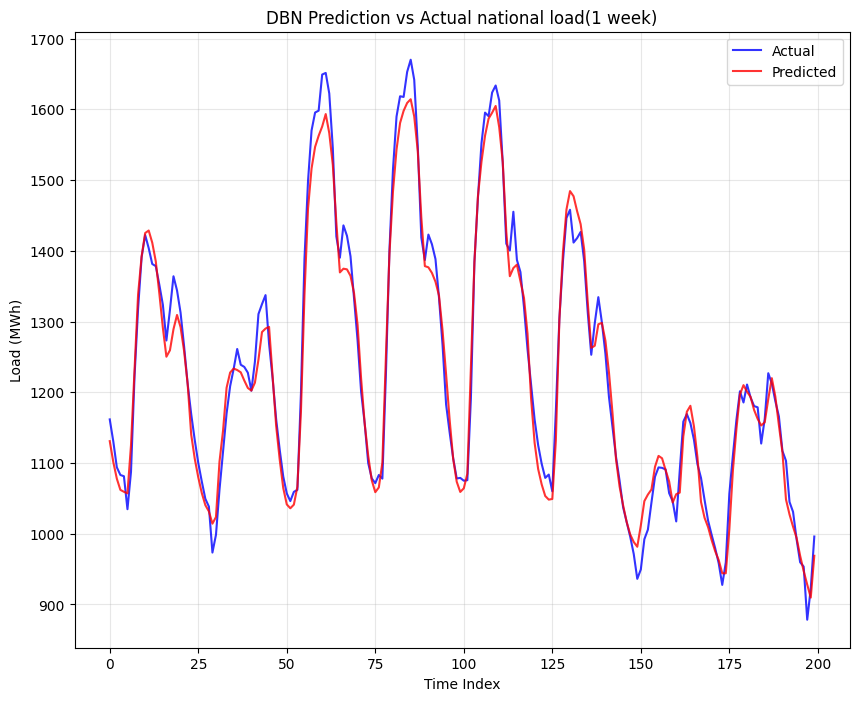
\includegraphics[width=\linewidth]{Chapters/images/results/DBN_predicted_vs_actual}
  		\caption{Predicted vs Actual load over a 1 week period of DBN}
  		\label{fig:dbnpredictedvsactual}
  	\end{minipage}
  	\hfill
  	\begin{minipage}[b]{0.48\linewidth}
  		\centering
  		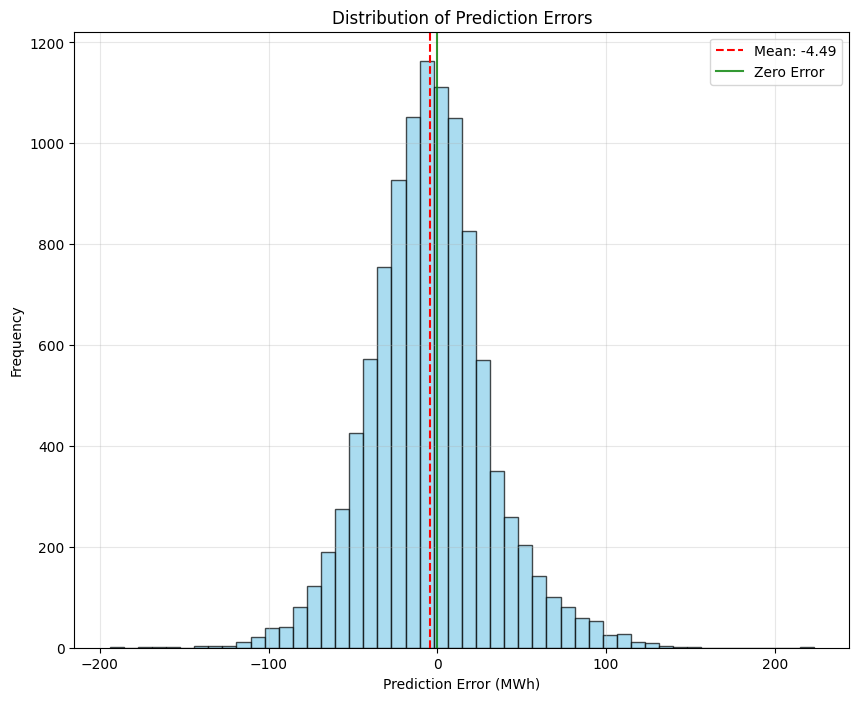
\includegraphics[width=\linewidth]{Chapters/images/results/dbn_error_distribution}
  		\caption{Distribution of prediction errors for the DBN model}
  		\label{fig:dbnerrordistribution}
  	\end{minipage}
  \end{figure}
  
  Figure \ref{fig:dbnpredictedvsactual} illustrates how the predicted load closely follows the actual load over a one-week period. The model’s errors are minimal, as highlighted in Figure \ref{fig:dbnerrordistribution}, which shows the distribution of prediction errors across all test cases. The error distribution approximates a normal distribution, with the majority of errors clustered near zero, indicating strong predictive performance.   
  \begin{figure}[h]
  	\centering
  	\includegraphics[width=0.5\linewidth]{"Chapters/images/results/dbn_validation loss"}
  	\caption{DBN model loss during training and validation}
  	\label{fig:dbnvalidation-loss}
  \end{figure}
 
 
 \subsection{CNN model results}
 
 The CNN model produced a Test MAPE of 2.74 however similar to the DBN values, with an $R^2$ value of 0.93. Table \ref{tab:cnn_performance_diff} contains the test and train results of the model. The comparison is meant to show if there was a possibility of an overfitting of the data.
 \begin{table}[h]
 	\centering
 	\caption{Performance Metrics of the CNN Model}
 	\label{tab:cnn_performance_diff}
 	\begin{tabular}{lccc}
 		\hline
 		\textbf{Metric} & \textbf{Training} & \textbf{Test} & \textbf{Difference} \\
 		\hline
 		MAPE (\%) & 1.4700 & 2.7414 & +1.2714 \\
 		MAE (Mwh) & 16.7129 & 33.0764 & +16.3635 \\
 		RMSE (Mwh) & 25.2818 & 46.8295 & +21.5477 \\
 		R$^2$ & 0.9827 & 0.9375 & -0.0452 \\
 		MSE & 639.1704 & 2192.9995 & +1553.8291 \\
 		\hline
 	\end{tabular}
 \end{table}
Similar to the results obtained for the DBN model (Section \ref{sec:dbn results}), the high $R^2$ values observed in the CNN model do not necessarily indicate overfitting. The elevated $R^2$ can be attributed to the inclusion of additional features generated during data preprocessing and feature engineering. As noted by Plevris et al. \cite{plevris2022investigation}, the $R^2$ value tends to increase with the addition of more features, even when some of these features do not have a direct correlation with the model’s output. Figure \ref{fig:cnnmodelloss} shows how the train and value loss change over the epochs. The image shows a smooth decline in the train loss, however the validation loss has a fluctuating loss that does not converge.
Figure \ref{fig:cnnpredictionvsactual} shows the prediction vs the actual output of the CNN model. The predicted load closely follows the actual load.
\begin{figure}[h]
	\centering
	\begin{minipage}[b]{0.46\linewidth}
	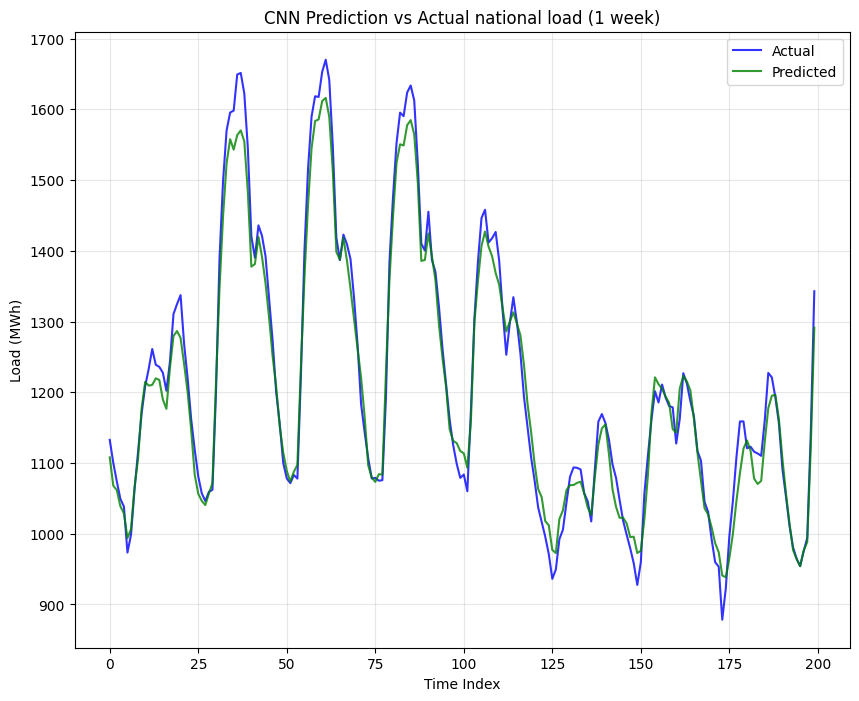
\includegraphics[width=\linewidth]{Chapters/images/results/cnn_predictionvsactual}
	\caption{The predicted and actual loading from the CNN model}
	\label{fig:cnnpredictionvsactual}
	\end{minipage}
	\begin{minipage}[b]{0.46\linewidth}
	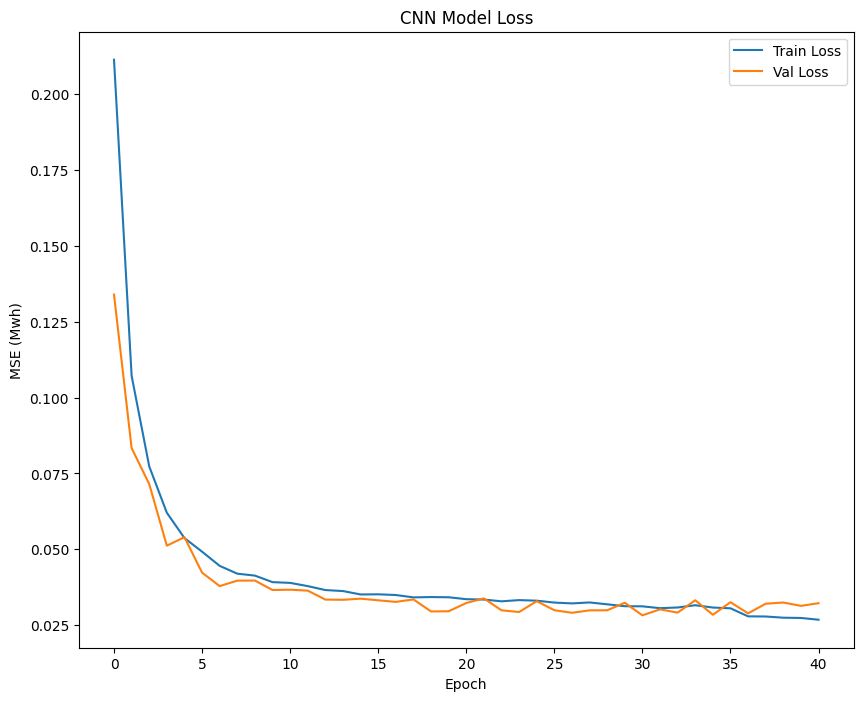
\includegraphics[width=\linewidth]{Chapters/images/results/CNN_model_loss}
	\caption{The CNN model validation and test loss against the epochs}
	\label{fig:cnnmodelloss}
	\end{minipage}
\end{figure}

\subsection{Hybrid Model Results: CNN LSTM}
 The hybrid model produced 
 \[
 b_t = \gamma (S_t - S_{t-1}) + (1-\gamma) b_{t-1}
 \tag{13}
 \label{eqn:877}
 \]



		\chapter{Discussion}

Here is what the results mean and how they tie to existing literature...

Discuss the relevance of your results and how they fit into the theoretical work you described in your
literature review.

		\chapter{Conclusions}

These are the conclusions from the investivation and how the investigation changes things in this field or contributes to current knowledge...

Draw suitable and intelligent conclusions from your results and subsequent discussion.

		\chapter{Recommendations}

Make sensible recommendations for further work.

		

\bibliographystyle{ieeetr}
\bibliography{Bibliography/References.bib}
		\appendix
		\appendix 
\chapter{Appendix 7\label{sec:appendixA}}
\begin{figure}[htbp]
	\centering % Centers the image and caption
	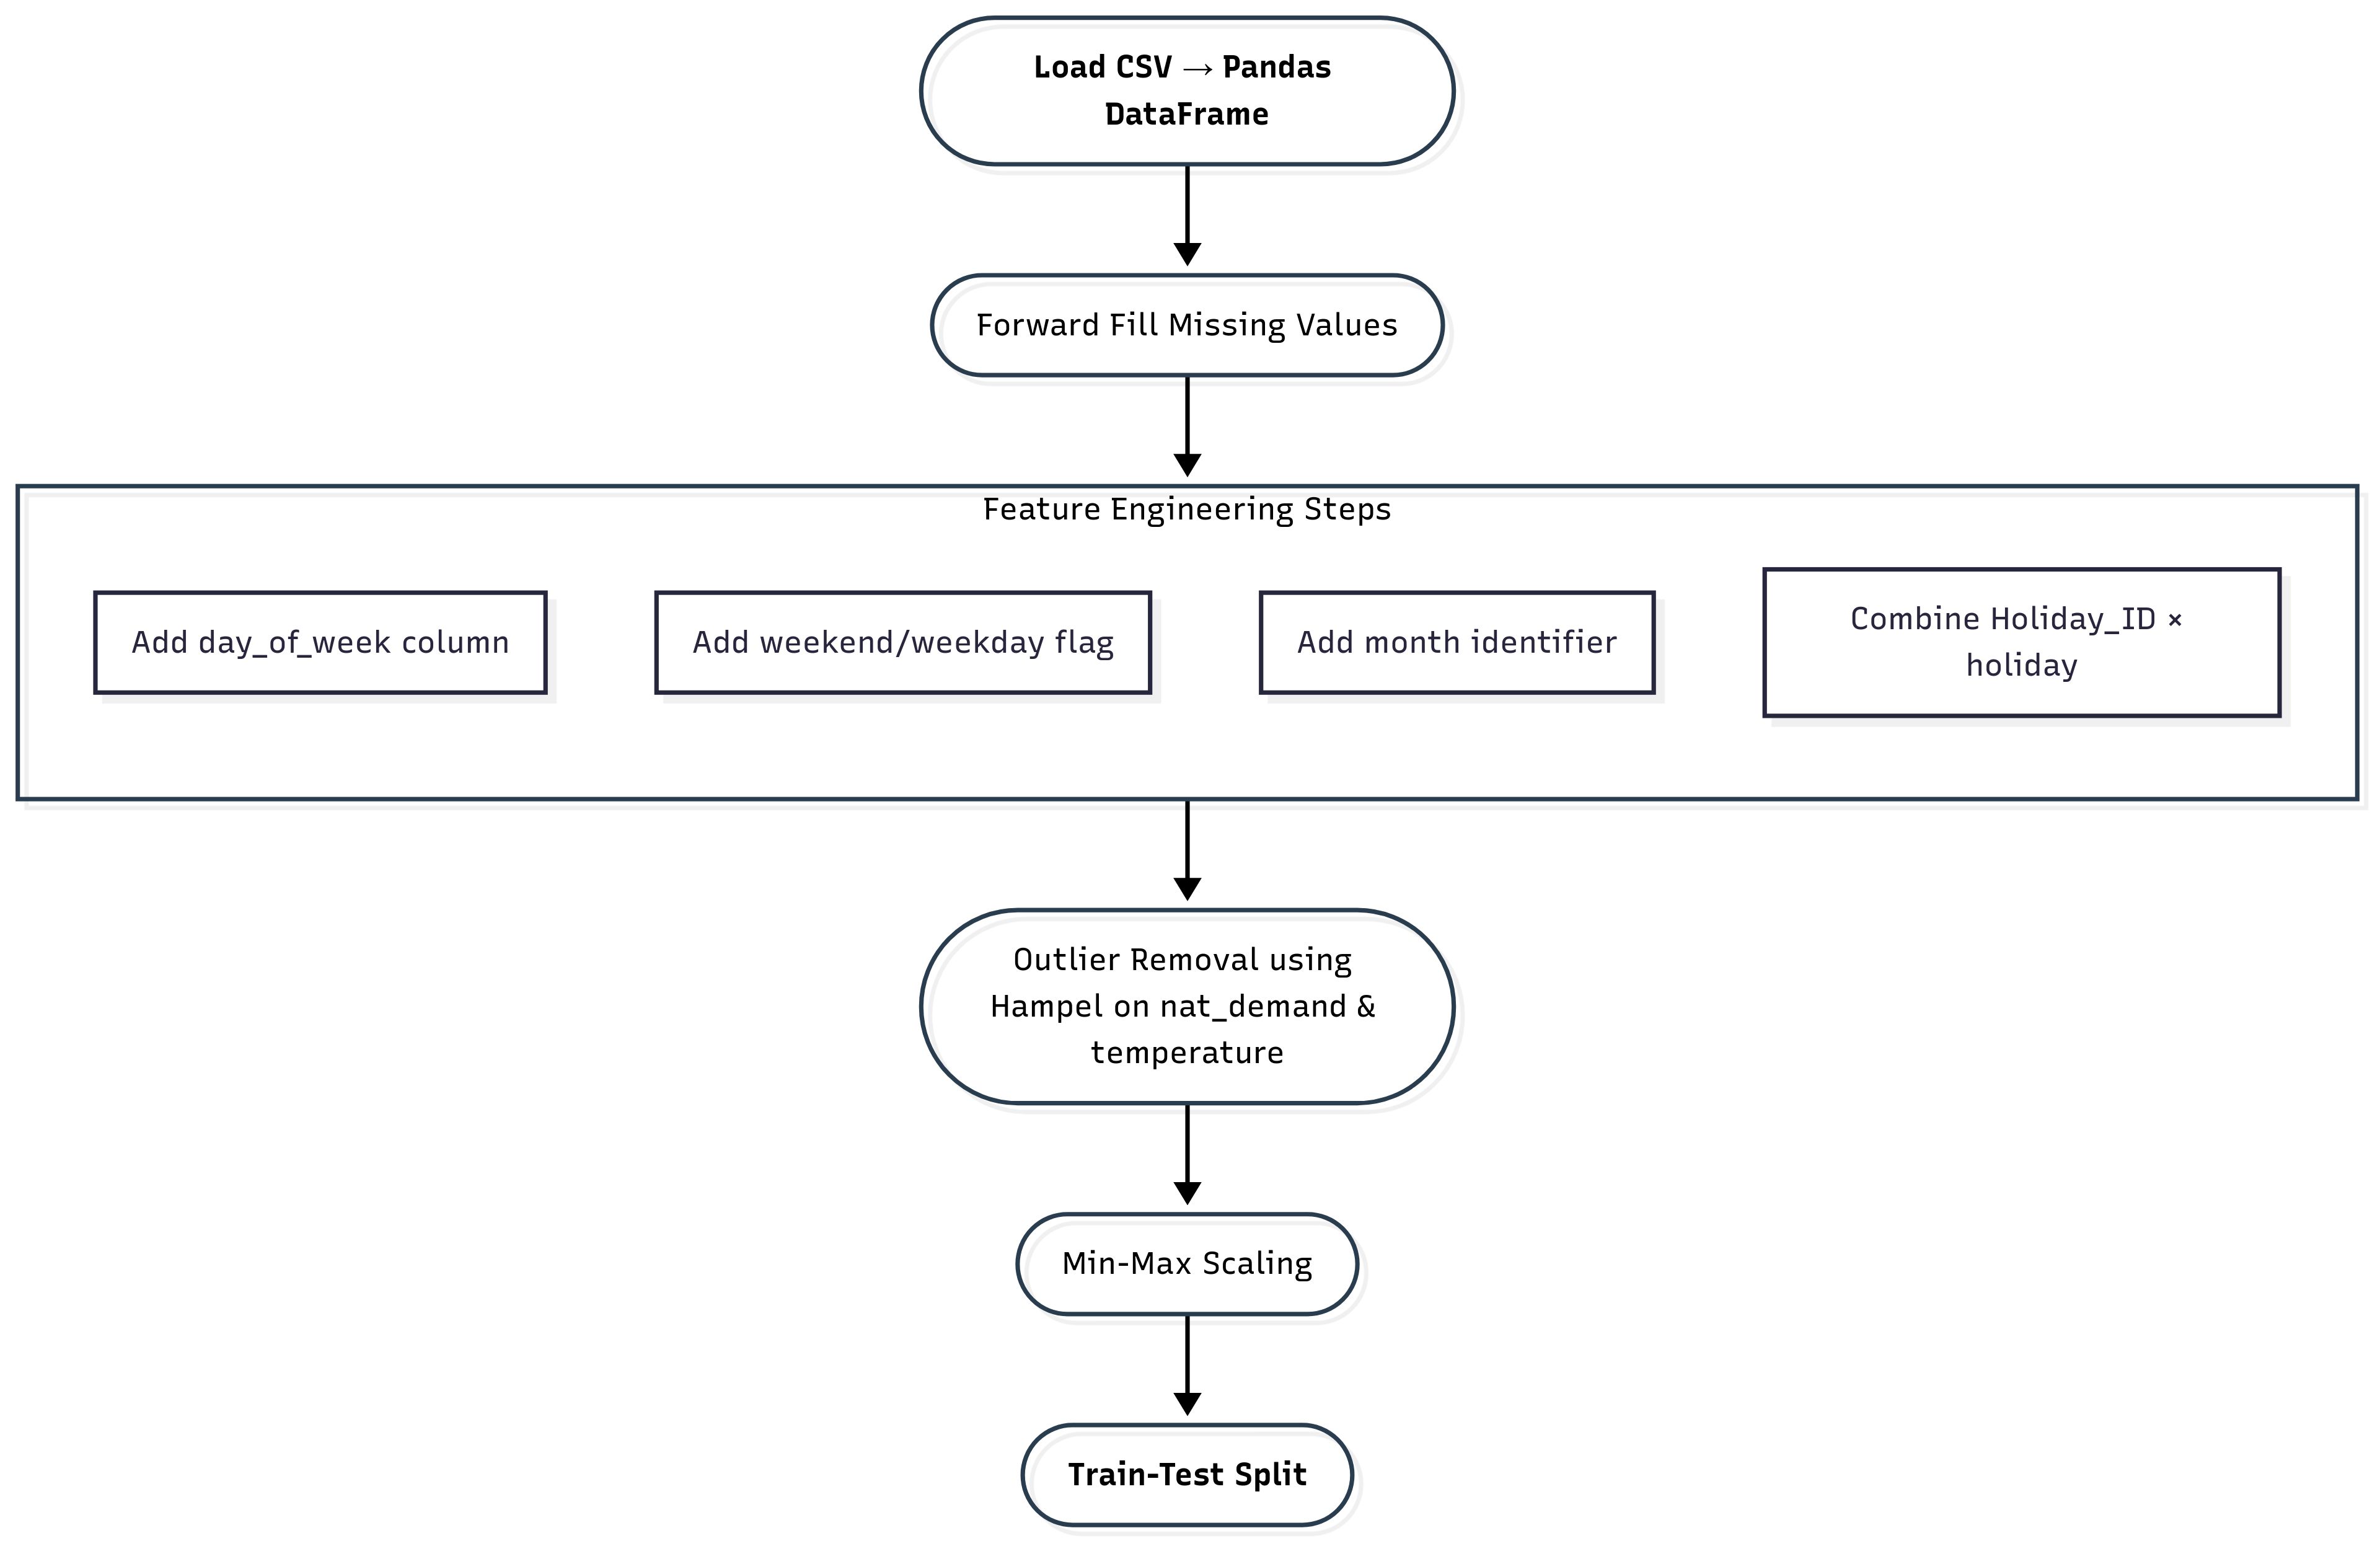
\includegraphics[scale=0.1]{Chapters/images/preprocess.png}
	\caption{The data preprocessing steps taken to process the data for model training}
	\label{fig:preprocessing_steps_flowchart} % For referencing the figure later
\end{figure}


\begin{figure}[htbp]
	\centering % Centers the image and caption
	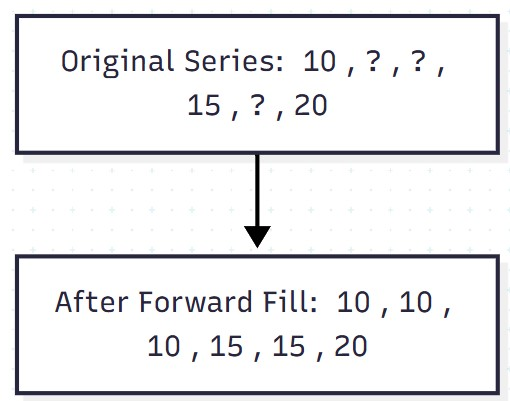
\includegraphics[scale=0.4]{Chapters/images/forward_fill.jpg}
	\caption{Forward Fill algorithm demonstration}
	\label{fig:forward_fill} % For referencing the figure later
\end{figure}
\begin{figure}[h]
	\centering
	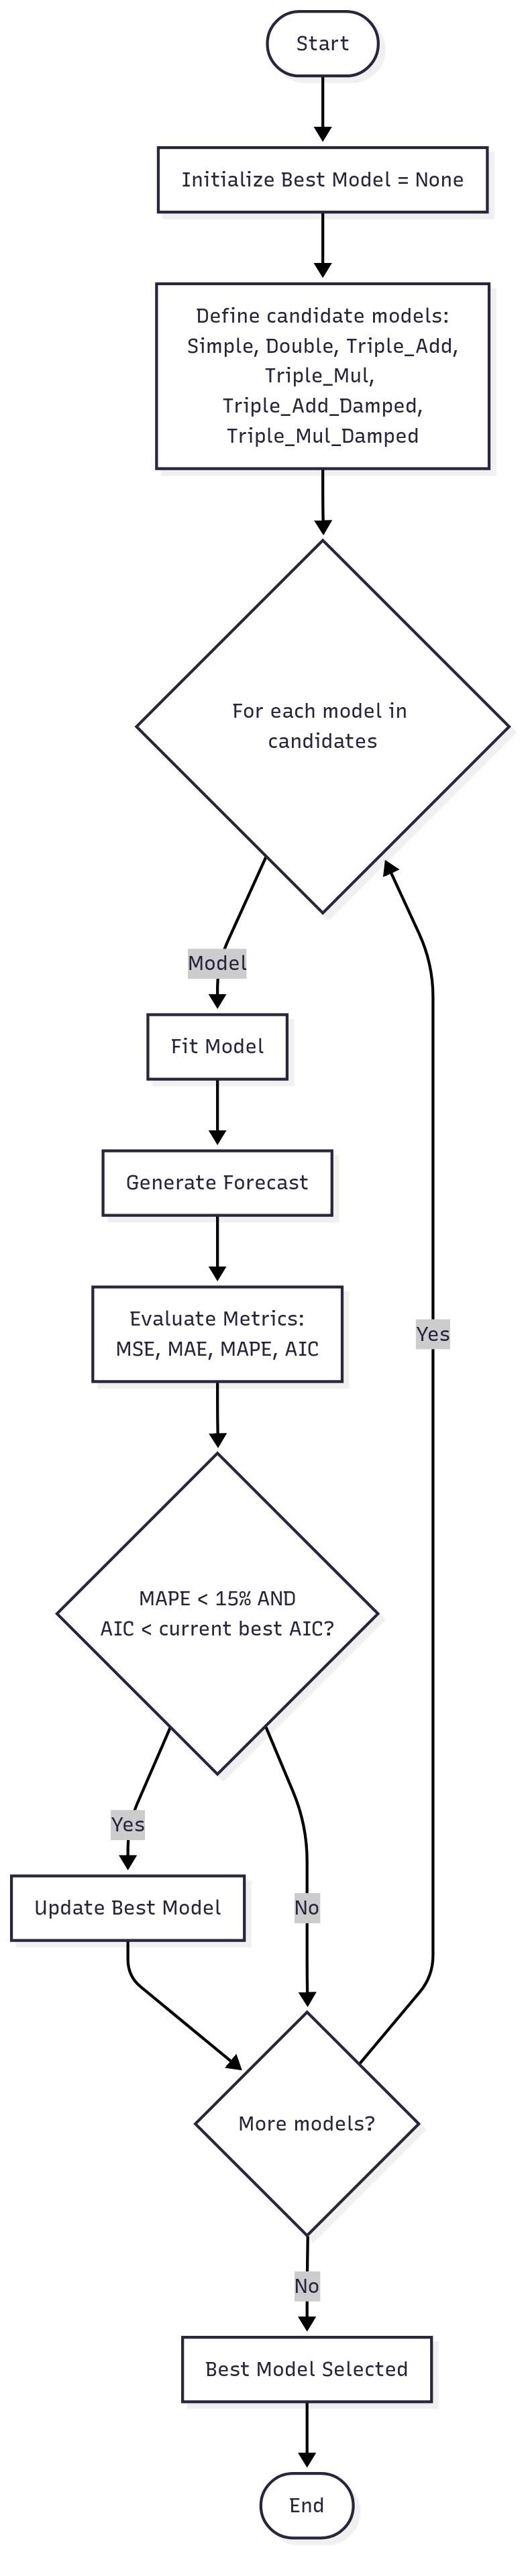
\includegraphics[scale=0.18]{"Chapters/images/exponentialsmoothingmodel.png"}
	\caption{Exponential smoothing model selection design choices.}
	\label{fig:exponential-smoothing-model-choice}
\end{figure}

\begin{figure}[h]
	\centering
	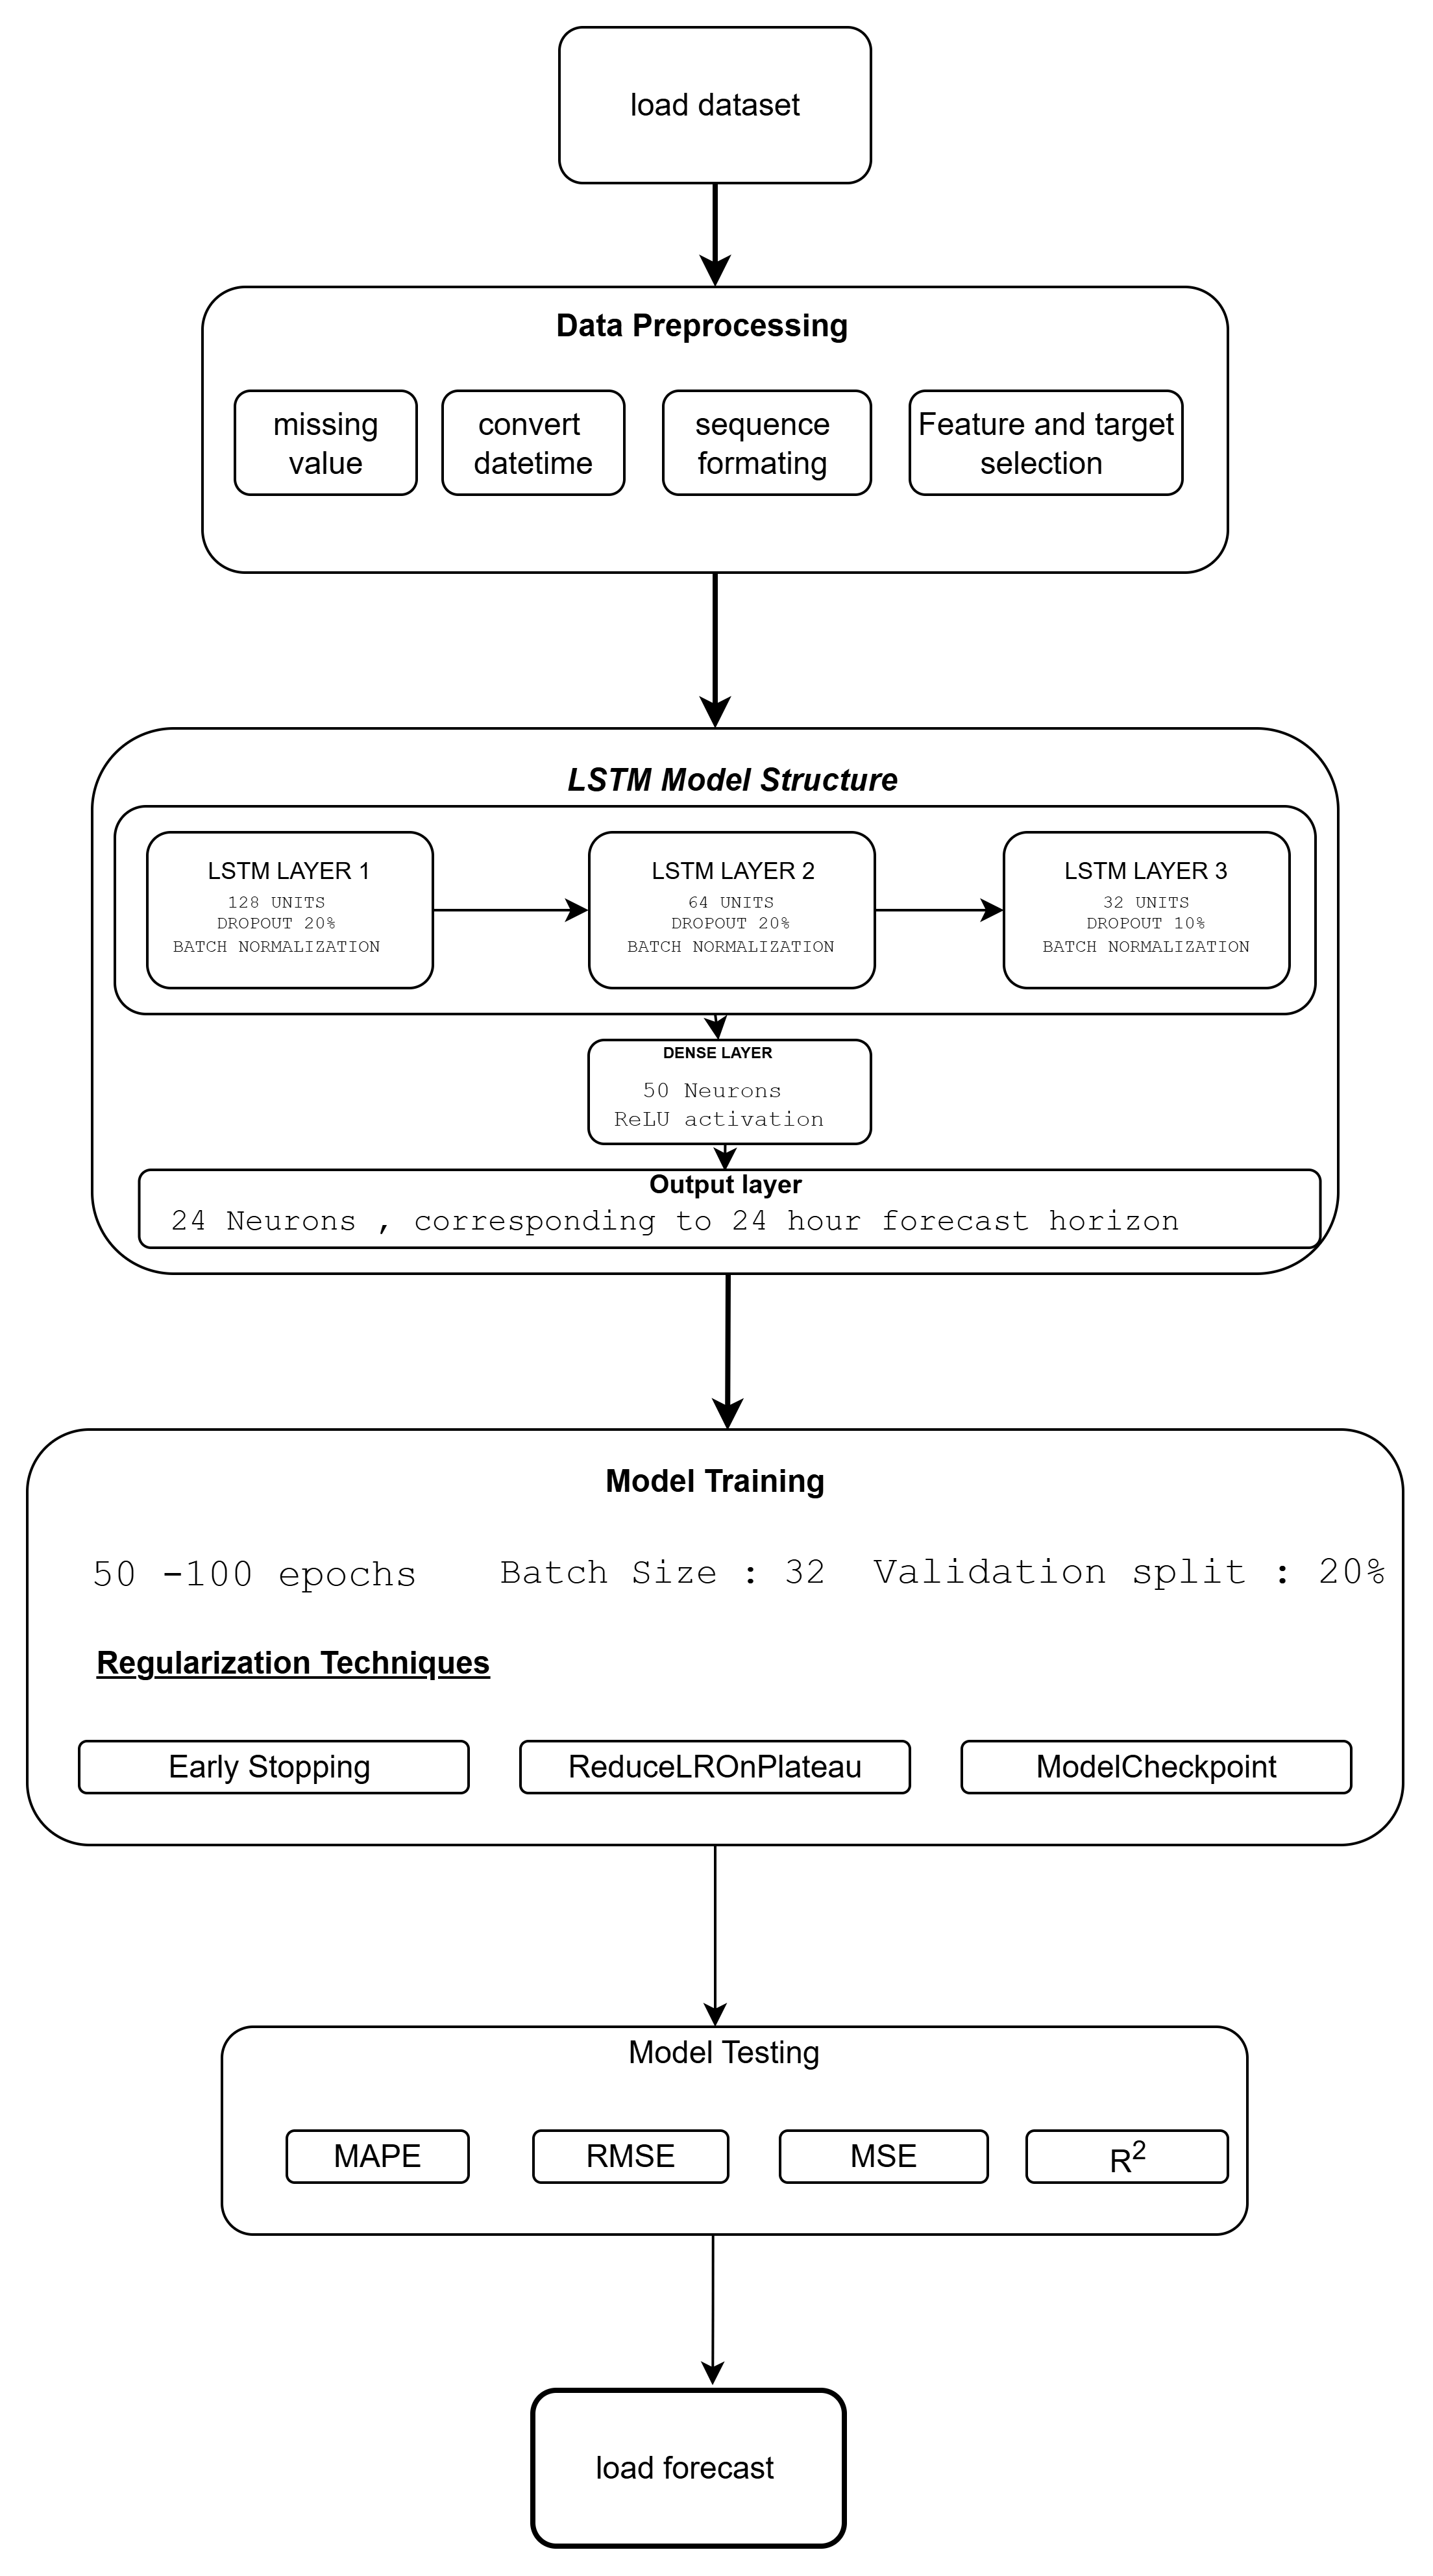
\includegraphics[width=0.7\linewidth]{Chapters/images/lstm_flowchart}
	\caption{full flowchart of the lstm model}
	\label{fig:lstmflowchart}
\end{figure}

		\chapter{Addenda}

\section{Ethics Forms}
	
\end{document}
